%\documentclass[11pt]{article}
\documentclass[print,ms]{nuthesis}
%\usepackage{times}

%\setlength{\textwidth}{6.5in}
%\setlength{\textheight}{9.0in}
%\setlength{\topmargin}{-.5in}
%\setlength{\oddsidemargin}{-.0600in}
%\setlength{\evensidemargin}{.0625in}

\newcommand{\secref}[1]{Section~\ref{#1}}
\usepackage{xcolor}

\usepackage[dvipdfm,%
bookmarks=true,%
bookmarksopen=true,%
bookmarksnumbered=true,%
bookmarkstype=toc,%
pdftitle={Derek Weitzel Thesis--Campus Grids},%
pdfsubject={},%
pdfauthor={Derek Weitzel},%
pdfkeywords={Weitzel, Grid, Campus},
%linktocpage=true,
linkbordercolor=white
]{hyperref}


%\newcommand{\doublespace}{\baselineskip0.34truein}
%\newcommand{\singlespace}{\baselineskip0.16truein}
%\newcommand{\midspace}{\baselineskip0.24truein}
%\newcommand{\midplusspace}{\baselineskip0.26truein}




%\usepackage{setspace}
\usepackage{algorithmic}
\usepackage{algorithm}

\usepackage{graphicx}
\usepackage{calc}
\usepackage{url}
\usepackage{listings}
\usepackage{subfig}
\usepackage{multirow}
\usepackage{bbding}
\usepackage{rotating}
\usepackage{array}

\newlength{\imgwidth}

\newcommand\scalegraphics[1]{%   
    \settowidth{\imgwidth}{\includegraphics{#1}}%
    \setlength{\imgwidth}{\minof{\imgwidth}{\textwidth}}%
    \includegraphics[width=\imgwidth]{#1}%
}



%\doublespacing

%\author{Derek Weitzel\\
%Computer Science and Engineering\\
%University of Nebraska--Lincoln\\
%Lincoln, NE 66588-0115\\
%dweitzel@cse.unl.edu
%       }
       
\begin{document}
\frontmatter
\title{Campus Grids: A Framework to Facilitate Resource Sharing}
\author{Derek Weitzel}
\adviser{Professor David Swanson}
\adviserAbstract{David Swanson}
\major{Computer Science}
\degreemonth{May}
\degreeyear{2011}

\maketitle

\begin{abstract}

It is common at research institutions to maintain multiple clusters.  These might fulfill different needs and policies, or represent different owners or generations of hardware.  Many of these clusters are under utilized while researchers at other departments may require these resources.  
This may be solved by linking clusters with grid middleware.  This thesis describes a distributed high throughput computing framework to link clusters without changing security or execution environments.  
The framework initially keeps jobs local to the submitter, overflowing if necessary to the campus, and regional grid.
The framework is implemented spanning two campuses at the Holland Computing Center.  We evaluate the framework for five characteristics of campus grids.  This framework is then further expanded to bridge campus grids into a regional grid, and overflow to national cyberinfrastructure.

%the framework is designed as lightweight, and leveraging existing security infrastructure.   All of these components are functional and are running research jobs in production.

\end{abstract}

%\newpage
\tableofcontents
\newpage
\listoffigures
\listoftables

% \doublespace
\mainmatter
\chapter{Introduction}
\label{sec:Introduction}

%\subsubsection* {The problem we have solved}

%\begin{itemize}
%\item
%Concentrate on making {\em this} assertion and {\em only} this assertion in a
%succinct set of 1 to 3 paragraphs 

%\item Department clusters waste power by being under utilized for significant portions of time.
%\item Researchers have peaks in usage and need overflow capacity.
%\item Move single core jobs around to idle clusters, freeing up space for MPI jobs.
%\item Users want a single execution environment.  This is an expressed goal of the Condor project.
%\item Increased utilization of a cluster can reflect well on the department.
%\item Use existing security infrastructure.

%\item
%A common mistake is to explain too much of the problem context first. Instead,
%state the problem essentially as a claim, and leave explanations supporting
%your claim to the next part, ``Why it is not already solved.''

%\end{itemize}

A computational grid is a hardware and software infrastructure that provides dependable, consistent, pervasive, and inexpensive access to high-end computational capabilities\cite{foster2004grid}.  A campus grid is a specialized grid where resources are owned by the same organization, though they can be in multiple administrative domains.  We further restrict our considerations to those campuses that have multiple computation resources.

A campus grid has become necessary to alleviate demand on newer parallel machines by moving single core jobs to other resources that have idle cycles, such as previous generations of parallel machines and idle workstations.  By moving the single core jobs, it can free the newest hardware for large parallel jobs that can benefit from better interconnects, larger and faster storage, and increased core count that are on the newest hardware.

A campus grid requires a framework for distributing computation among independent clusters within a campus.  A campus typically contains multiple compute clusters that are independently administered.  A campus grid's purpose is to increase the processing power accessible to users by connecting compute resources.   By \mbox{offloading} jobs from clusters that are full to idle clusters, they can increase utilization.  Additionally, the users can benefit by increased processing power.  

The framework described in this thesis is used to create a production campus grid.  The campus grid includes technology to allow  participation in the campus grid by clusters that use several schedulers, and uses production quality software integrated into a solution that is deployed at several clusters in the U.S.  The campus grid framework provides a method for users to run jobs transparently on available distributed resources on the campus grid.  Further, it can expand beyond the campus and onto other campuses by simple configuration changes.

At the Holland Computing Center (HCC) \cite{hccwebsite} at the University of Nebraska -- Lincoln, I created a campus grid, the HCC Campus Grid, that spans two clusters and can overflow onto the national grid infrastructure.  The HCC Campus Grid borrowed concepts and techniques from earlier campus grids and a national grid, the Open Science Grid (OSG).  The OSG focuses on High Throughput Computing (HTC), concentrating on tasks that require as much computing power (throughput) as possible over long periods of time \cite{gridbook-htc}.  The HCC campus grid also focuses on HTC tasks.  

The HCC Campus Grid bridges clusters and the national infrastructure while running production processing jobs from on-campus researchers. Since the beginning of 2010 to March 2011, we ran 8,151,607 jobs for 9,022,655 hours on the HCC Campus Grid infrastructure.

The HCC Campus Grid differs from existing campus grids by building an expanding pool of resources for the users.  Other campus grids are limited to available resources on the campus or in a regional grid.  The HCC Campus Grid can transparently submit to ever increasing distant resources.  Figure \ref{fig:circleresources-intro} describes the widening available resources to users.  The HCC Campus Grid will first attempt to run at the local cluster, then campus clusters, and finally out to other campus grids or a national grid.

\begin{figure}[h!tbp]
\begin{center}
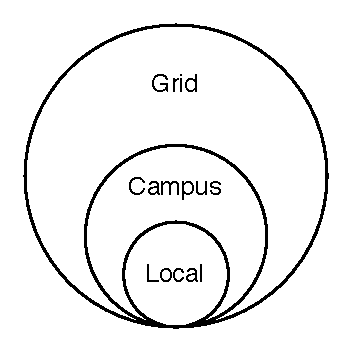
\includegraphics[scale=0.8]{images/BWCircles}
\caption{Widening Circle of Resources}
\label{fig:circleresources-intro}
\end{center}
\end{figure}

Building a campus grid represents a significant commitment for both users and resource providers, which should be 
evaluated against the benefits.  Other Campus grids may provide one or two of the listed benefit, but the HCC Campus Grid provides them all in a cohesive framework.  The primary benefits of the HCC Campus Grid are:
\begin{itemize}
\item \textbf{Resource sharing}: An HTC-based approach focusses on using all resources effectively.  Resources are 
typically bought for peak, not average, usage; utilizing the idle time across the entire campus improves 
the value of the investment.
\item \textbf{Homogeneous interfaces to multiple resources}: Moving researchers from one resource to another results in 
a (possibly large) upfront cost in time and energy.  By providing a homogeneous interface across the campus, 
researchers can quickly utilize new resources without the pain of migration.
\item \textbf{Independence from any single computational resource}:  It is expensive to provide highly available 
resources.  If a researcher does not rely on a specific single cluster, individual cluster downtimes have a smaller impact.  This 
reduces the need for high levels of redundancy and stretches the campus computing budget further.
\end{itemize}

An obvious requirement for campus grids is having multiple resources on campus.  However, this is not sufficient for 
resource providers--the resources should also be interchangeable.  A grid composed of a single AIX cluster, Linux 
cluster, and Windows cluster, will likely never see any resource pooling or sharing.  This does not necessarily imply 
the resources need to be identical--complete homogeneity is typically impossible due to individual resource 
requirements or ownership.  Often it is undesirable to have homogeneity as resources can fulfill different 
resource requirements such as large memory or local scratch space.

A mistake in campus grids is to focus on the infrastructure for pooling resources without similarly engaging and 
supporting the activities of users.  An analogy can be made to fluid: if there is a sink (resources) with no source 
(user jobs), the flow quickly stops, and the campus grid is forgotten.  Personnel investment must be made to engage 
the user community.  Even before this investment is made, a campus should identify whether the on-campus scientific 
computing has a significant portion of tasks that can be converted to HTC workflows.  Prioritization should be applied 
so the users with the simplest workflow and the most to benefit are converted first.  Tasks with the following 
characteristics should typically be avoided:

\begin{itemize}
\item \textbf{Large scale (multi-node) MPI:} Require specific tunings to the given \mbox{resource}.
\item \textbf{Multi-day jobs:}  Shared resources often need to be reallocated quickly back to the owner, meaning these jobs are 
unlikely to complete.
\item \textbf{Sensitive data or software:}  Tasks with sensitive (for example, HIPPA-protected) data may have legal boundaries 
preventing distribution.  Software with strict licenses may also be illegal to use across the grid.
\end{itemize}



%As the speed of innovation in computing increases, it is common for a campus to have multiple generations of clusters.  These clusters are commonly bought as independent systems, not meant to share work between them.  This causes users to flock to the newest generation hardware, hoping to increase the performance of their application.  This movement of users leads to under utilization of older hardware, and increased demand on the newest.

%This is just one of many situations that would cause users to underutilize hardware.  Other situations could be:

%\begin{itemize}
%\item \textbf{Departmental clusters:}  Each department has a dedicated cluster.  This cluster specialization can cause under utilization when department researchers are not using the resources.
%\item \textbf{Peaks of usage:} In general, users have peaks to their usage around deadlines.
%\item \textbf{Parallel jobs:} While a cluster is draining nodes for a large parallel job, the cluster could fill those drained slots with pre-emptable usage.
%\end{itemize}





%\subsubsection* {Why the problem is not already solved or other solutions 
%are ineffective in one or more important ways}


%\item
%Your new idea need not solve every problem but it should solve at least one
%that is not already solved







%\item 
%A common solution to linking clusters is condor flocking.  Flocking requires every cluster to run condor daemons on their nodes.  

% Last case, since it's simalar to mine.
%Several universities have approached the problem utilizing condor flocking.

%\item
%This is the place to provide a succinct description of the problem context
%giving enough information to support the claim that a problem exists, made in
%the preceding problem declaration.





%\subsubsection* {Why our solution is worth considering and why is it effective
%in some way that others are not}



There have been several methods to create a distributed campus grid.  They all use some technology to distribute and schedule the jobs on the grid.  Some methods for distribution are commercial products such as  the meta scheduler Moab \cite{website:moabgrid}.  Others are translation layers between a generic description language and a scheduler, such as Globus \cite{foster1997globus}, CREAM \cite{andreetto2006cream}, and ARC \cite{eerola2006roadmap}.  Still others are entire resource managers that can span multiple clusters like Condor \cite{thain2005distributed}.  Each of these solutions can be utilized to create a campus grid, but they all have drawbacks that are detailed in \mbox{\secref{sec:others}}.




  
% Unnecessary sentence?
%The campus grid is used in production at the University of Nebraska, connecting two geographically separate clusters.  Users can utilize the campus grid by submitting to one of the connected clusters, while their jobs run on either.  The jobs are transported with their input files to a execution sandbox on the worker node.  Further, the campus grid expands beyond Nebraska, peering with the Purdue campus grid.


% This will largely be from CHEP paper
\chapter{Background}
\section{Characteristics of Campus Grids} \label{sec:attributes}
In this section, we explore five characteristics of HTC-centric campus grids. While the list is not exhaustive, these are foundational characteristics of campus grids.  We've 
found that campus grids can be characterized by how they approach trust relationships, job submission, resource 
independence, accounting, and data management.


\subsection{Trust Relationships}
A campus grid must have an acceptable trust model in order to succeed.  A trust relationship enables 
a resource provider to grant campus users controlled access to the resource, and may be established through 
 sociology and/or technology-based security methods.

In the OSG, the trust model used is designed to be homogeneous and to meet the most stringent requirements of 
all participating sites.  The implementation involves using Globus's Grid Security Infrastructure (GSI) with Virtual Organization Membership Service (VOMS)  
attributes, a Public Key Infrastructure (PKI) extension \cite{farrell2002rfc3281}.  The GSI model is widely 
accepted, allowing the OSG to participate in the Worldwide LHC Computing Grid (WLCG) \cite{wlcg}.  FermiGrid, located at the Fermi National Accelerator Laboratory in Batavia, Illinois, uses GSI authentication on its campus grid. 
While it provides a highly secure, decentralized authorization model,
it is more difficult for end users compared to traditional username/password 
authentication.  Thus, campus grids may be motivated to use alternate trust models.

On-campus resource providers may have a higher implicit degree of trust than at the national level due to 
sociological reasons.  This trust is partially based on locality--it is easier to establish a working relationship 
with a colleague locally on campus than 1000 miles away.  Additionally, a national lab such as Fermilab is higher profile 
than most universities and therefore requires stronger trust relationships to maintain security and accountability.

Security requirements on some university campuses are simply less stringent than that of federal labs.  A campus may 
not have strict policies governing user job separation or traceability requirements.  Some campus clusters may be 
satisfied with running any job originating from elsewhere on the campus to an unprivileged account.  When a job crosses 
domains (from local cluster to across campus, or from campus to the national grid), it must 
satisfy the security requirements for the destination domain.  Thus, if a campus grid would like to bridge to the 
national grid, users must be able to associate GSI credentials with their jobs.

A technical reason for different trust relationships between campuses and larger grids is the location of user 
job submit hosts.  Unlike the OSG, where users can submit jobs from any worldwide host, campus users often submit from 
a few trusted campus resources.  If limited to a few well-managed hosts, IP-based security may be sufficient for 
campuses, as the security such as username and password is applied to submit hosts rather than cluster entry points.




\subsection{Job Submission}
In order for a HTC-oriented campus grid to function, users need a usable job submission interface.
The Globus Toolkit \cite{foster1997globus} provides the Globus Resource Allocation Manager (GRAM) interface for job 
submission and corresponding clients.  The GRAM layer abstracts the batch system; the 
remote user interacts with the site's GRAM install and GRAM converts these actions into batch system commands at the destination.
The GRAM interface is used by the OSG at the scale of over 100 million jobs a year.  It abstracts many batch system constructs, and is also used 
on the TeraGrid to submit larger jobs running on hundreds or thousands of cores.  While GRAM can be used directly, 
users almost exclusively prefer to interact with it via Condor-G  \cite{frey2002condor} , which provides a batch 
system interface on top of GRAM.  FermiGrid relies on Condor-G submission to GRAM for job submission.

An abstraction layer like GRAM introduces a new user experience (even if Condor-G is used), requiring new expertise. An 
alternate approach is to uniformly use batch system software that can interact with multiple instances of itself.  By 
linking resources at the batch system level rather than adding an abstraction layer on top, we improve the user 
experience--users no longer need to learn additional tools.  The client tools do not need to translate errors across 
different domains, easing a common source of frustration in the grid.  When Condor-G is used, we have a batch-system 
interface abstracting an API which, in turn, abstracts remote batch systems; thus, error propagation is extremely difficult.  
In some campus grids described in \secref{sec:others}, 
resources are linked through use of a common batch system, Condor, through a mechanism Condor refers to as 
``flocking".  A hybrid between Condor-only and GRAM is given by GlideinWMS \cite{sfiligoi2008making}.

In our observations, the closer the grid user experience is to the batch system user experience, the more likely a 
user will adopt the campus grid.



\subsection{Resource Independence}
Compared to a corporate IT environment, one unique aspect of universities is the diversity of management of 
computing 
resources.  On a campus, several distinct teams may manage distinct clusters due to campus 
organization or ownership.  Management of resources may be divided by college, department, or lab.  One 
characteristic of campus grids is the independence of resources--the level of decision-making delegated out to 
the resource providers.

The simplest campus grids can be formed by requiring all clusters on campus to run the same batch system and linking 
batch system instances--Grid Laboratory of Wisconsin's (GLOW) use of Condor is an example.  Every cluster in GLOW runs the Condor batch system, 
providing a common interface.  System administrators are not free to choose their own batch systems if they want to 
participate in this grid (participation is voluntary, and participants obviously believe the benefits of GLOW 
membership outweighs this drawback).  It may be desirable for a specialized cluster to have a distinct batch system  
from the rest of the campus; resource independence allows the cluster owners to best optimize their resource to suit 
their needs.

Resource independence comes at a cost to the end-user.  Extremely heterogeneous resources can be difficult to 
integrate at the software level--an application compiled for Linux will not be compatible with Windows.  Some guarantees 
about the runtime environment or other interfaces need to be clearly articulated and agreed upon to prevent frustration.  Differences 
that are unavoidable or are expected to be handled by the user should be clearly expressed to the user \cite
{raman2002matchmaking}.  At the OSG level, we have found the users often frustrated by the amount of heterogeneity, especially unexpected heterogeneity, compared to using a single site or a grid with a smaller number of sites \cite{zvada2010cdf}.


\subsection{Accounting}
Accounting may not seem to be an important grid characteristic--it certainly isn't required for 
users to successfully run a job.  However, it is critical for the long-term health of the campus grid as it provides a quantitative 
measurement of the grid's value.  One economic model for the grid is for resource providers and users to ``barter" for computing hours as reported by accounting services. 

Accounting systems do not need to be technically advanced.  Most batch systems provide a local accounting 
system.  The most basic method is for each cluster to parse these logs into a CSV file per cluster, and to 
build an Excel spreadsheet out of the aggregated files.  This is functional, but painful when statistics are needed 
more than once a month.  Most batch system vendors sell accounting systems usable for multiple clusters, provided all 
clusters involved use the same batch system.

Many research computing centers have written their own accounting systems at some point; most implementations are in 
the style of  PHP-based web interface on top of a custom database, again fed by custom log-parsing scripts. Both the 
OSG and TeraGrid have spent effort on accounting software to suite their needs.  The OSG's Gratia \cite{gratiaweb} is 
designed to be reusable by other organizations, and is in use at the FermiGrid campus grid.

Any site-local accounting systems--homegrown, vendor provided, or designed for the national 
grids--can work at the campus grid level as long as they can answer the following questions for a given time 
period:
\begin{itemize}
\item How much computing resource was consumed overall?
\item How much computing resource did a specific user/group consume?
\item How much computing resource did a specific user/group consume on resources they did not own; i.e., 
�how much did I get from resource sharing?�
\item How much computing resource did a specific cluster provide?
\item How much computing resource did a specific cluster provide to groups that did not own it;  i.e., �how 
much did I give away due to resource sharing?�
\end{itemize}




\subsection{Data Management}
Scientific data management presents two challenges for research computing centers: volume of data and archival 
requirements.  The data volume is often larger than a single scientist can keep on their personal systems, and 
archiving requires expertise outside their field.

Distributed computing can present an additional challenge: managing data location.  Data access costs may be 
variable between different resources on a grid, or required data may simply be unavailable at some locations.  A simple 
solution is to export the same file system to all resources, hiding data locality from the user.  Unfortunately, this 
solution breaks down outside the campus since the file system would need to be accessed from outside campus, which can significantly hurt performance and increase administration cost on other campuses.   A single file system solution may not work in highly-distributed campuses as well.

More complex solutions include declaring data dependencies for jobs explicitly inside the job 
submissions (gLite WMS \cite{andreetto2008glite}, Condor), promoting data to be a top-level abstraction equal to jobs (Stork \cite
{kosar2005stork}), or promoting data to be the central concept above jobs (iRODS \cite{irodswebsite, 
rajasekar2007irods}).  The Compact Moun Solenoid (CMS) experiment's model separates the data management and job submissions systems, allowing the job 
submissions to simply assume all data is available (CMS PhEDEx \cite{phedex}).

While any system can be used for campus grids, the examples we consider in Sections \ref{sec:others} and \ref
{sec:hcc} either export a file system or utilize the tools from the job submission system.  The addition of a separate 
data management system often presents complexity to the users.  In some situations, it is easier for the user to not use distributed computing rather than deal with a complex data system.
Distributed computing is the cheaper alternative.  However, we note iRODS is an increasingly popular option and may 
have significantly decreased the operational cost of data management systems.


\section{Background}
\subsection{High Throughput Computing}
High Throughput Computing (HTC) is defined as tasks that require as much computing power (throughput) as possible over long periods of time \cite{gridbook-htc}.  This is in contrast to High Performance Computing (HPC), where users are concerned with maximizing instantaneous resources and response time.  HTC workflows are usually ensembles of independent single processor jobs with no communication between them.  This is not to say there isn't coordination; many workflow managers can utilize HTC to solve complex problems with many steps.  

As there is no communication between the jobs in a given task, they can be distributed across multiple resources.  This increases 
throughput, the end-goal of HTC.  HTC can use pooled resources mostly interchangeably and as such is well suited to 
distributed and grid computing models.  The OSG has demonstrated its technologies are successful; in Q4 2010, the OSG 
averaged over 400,000 jobs and a million computational hours a day using HTC.


\subsection{Condor}
Condor was developed at the University of Wisconsin--Madison.  An overview from \cite{thain2005distributed}:
\begin{quotation}
Condor is a high-throughput distributed batch computing system.  Like other batch systems, Condor provides a job management mechanism, scheduling policy, priority scheme, resource monitoring, and resource management.  Users submit their jobs to Condor, and Condor subsequently chooses when and where to run them based upon a policy, monitors their progress, and ultimately informs the user upon completion.  
\end{quotation}

An important technology used in Condor is the Classified Advertisement (\mbox{ClassAd}) mechanism.  ClassAds are the language that Condor uses to communicate between daemons and for matchmaking \cite{raman1998matchmaking}.  A ClassAd is a list of keys and values, where the values can be strings, numbers, or expressions.  All resources are described by ClassAds.  Job ClassAds have attributes such as log file, output, input, and job requirements.  Resource ClassAds have attributes such as  requirements to run on the resource, ownership, and policies.  ClassAds are used for matching jobs to resources by evaluating requirements of both the jobs and the resources.

Another component of Condor is the grid computing agent Condor-G \cite{frey2002condor}.  Condor-G communicates with Globus \cite{foster1997globus} sites.  Condor provides job submission, error recovery, and creation of a minimal execution environment.  Along with Condor-G, Condor can also submit jobs to other systems including Amazon EC2 \cite{amazonec2} and PBS \cite{pbstorque}.

Condor categorizes jobs by \texttt{universe}.  A \texttt{universe} in Condor specifies how the job should be handled.  The simplest example is the \texttt{vanilla} \texttt{universe}.  In this \texttt{universe}, the job is handled as a single executable, with input and output, that will exit when the job has completed.  When the \texttt{universe} is \texttt{grid}, this means that the job will be translated to another submission method.  The other submission methods could be a Globus GRAM submission, or as used in this thesis, as a PBS job submission.

Commonly used Condor daemons and their functions are described in Table \ref{table:condordaemons}.

\begin{table}
\centering
\begin{tabular}{| l | l |}
\hline
Daemon & Function \\
\hline \hline
\texttt{condor\_master} & Maintains Condor daemons   \\ \hline
\texttt{condor\_collector} & Information Provider \\ \hline
\texttt{condor\_schedd} & User Job Queue \\ \hline
\texttt{condor\_negotiator} & Scheduler: Matches jobs with resources \\ \hline
\texttt{condor\_startd} & Execution manager.  Runs on the resource \\ \hline
\end{tabular}
\caption{Condor Daemon Functions} \label{table:condordaemons}
\end{table}

\subsection{Open Science Grid}
The Open Science Grid (OSG) \cite{pordes2007open} is a national cyber infrastructure consortium that provides dedicated and opportunistic use of computation and storage resources consisting of nationally distributed universities and national laboratories. The OSG provides infrastructure, services, software, and engagement to the users.  

The OSG Production Grid provides a common interface to computing and storage resources: Globus and Storage Resource Manager (SRM)/GridFTP respectively.  Access to resourcesis provided by an OSG client.  Both Globus and SRM/ GridFTP were developed by consortium members and are included into the OSG packaging.  Many software tools have been contributed to the OSG software stack such as Condor and the Berkeley Storage Manager \cite{Bestman}.

A typical OSG site has a compute element that can run jobs and a storage element that can store data.  The storage element is both physically close and tightly coupled to the compute element in order to minimize latency for data.  Since most sites have their own storage element, they are used to stage data into and out of the site.

A user will install the OSG Client tools and submit to the sites.  The OSG tools will also include applications that can be used to stage data to the storage elements.  A user only needs a valid OSG certificate to access the grid resources.

The OSG is organized into groups of users called Virtual Organizations (VO's).  These VO's help users to run on the grid, as well as provide organization to many thousands of researchers.  Additionally, the VO can sign member's certificates to help sites identify users as belonging to the VO.  


% Do we need this?  Probably not, this is what the paper is about.
%\subsection{Campus Grids}






%\begin{itemize}
%\item
%A succinct statement of {\em why} the reader should care enough to read the
%rest of the paper.
%\item The framework described in this paper is designed as a modular framework that will allow clusters to overflow onto each other and to the grid.  This framework requires running condor on only one node in the cluster.  Each job that comes from another cluster will go through the default scheduler, whether it's PBS, SGE, or LSF.

%\item
%This should include a statement about the characteristics of your solution to
%the problem which 1) make it a solution, and 2) make it superior to other
%solutions to the same problem.

%\end{itemize}


%\subsubsection* {How the rest of the paper is structured}


\section{Thesis Overview}
The rest of this thesis first discusses technology to create campus grids as well as existing campus grids in
Chapter \ref{sec:RelatedWork}, and then describes our implementation in
Chapter \ref{sec:Implementation}. Chapter \ref{sec:Evaluation} describes how we evaluate
our system and presents the results. Chapter \ref{sec:Conclusion} presents our
conclusions and describes future work.


\chapter{Related Work}
\label{sec:RelatedWork}

%\subsubsection*{Other efforts that exist to solve this problem and why are they
%less effective than our method}

\section{Technology to Create a Campus Grid}

%\item
%Resist the urge to point out only flaws in other work. Do your best to point
%out both the strengths and weaknesses to provide as well rounded a view of how
%your idea relates to other work as possible

\subsection{Globus} \label{sec:globus}
Globus GRAM is a translation layer between a standard defined Resource Specification Language and the local resource manager.  It has been very successful and has a large install base.  Globus also has deep integration with standard grid authentication methods such as PKI.

Placing Globus gatekeepers on each cluster allows jobs to be submitted to each cluster without modifying the underlying batch system.  This requires a higher layer of abstraction over the Globus gatekeepers to optimally balance load between clusters.   
Globus GRAM implements the Grid Security Infrastructure (GSI) security that is inconsistent with most existing campus security architectures such as LDAP \cite{howes1997ldap} authentication or Kerberos \cite{steiner1988kerberos}.  It does not provide a method for transparent execution on other clusters: each submission must target a specific execution resource.  Therefore, there is no overflow capability in Globus, which experience on the OSG has shown is important to users.

\subsection{Condor Flocking} %\label{sec:flocking}
A single software solution is Condor.  Each resource can run Condor on their clusters and `flock' \cite{epema1996worldwide} to each other.  In this solution, jobs may not be balanced on each resource due to Condor's greedy scheduler algorithm, but they will find any idle slots available on the resources.  

\begin{figure}[h!t]
\centering
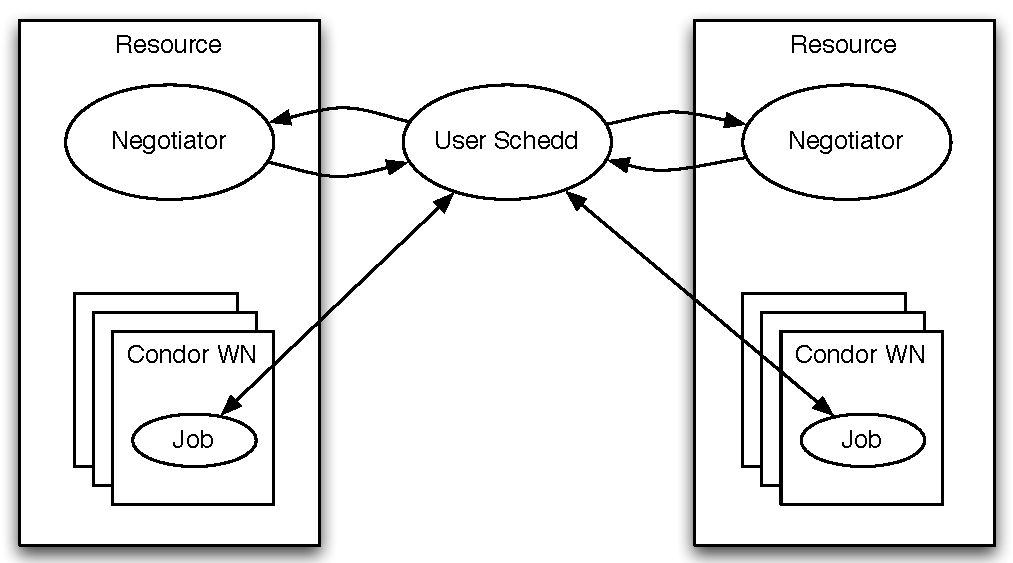
\includegraphics[scale=0.8]{images/Flocking}
\caption{Overview of Flocking}
\label{fig:Flocking}
\end{figure}

Flocking jobs is accomplished by a multi-step process, displayed in Figure \ref{fig:Flocking}.  First, the \texttt{condor\_schedd} reports to the remote \texttt{condor\_collector} that it has idle jobs available to run.  During the next negotiation cycle, the remote \texttt{condor\_negotiator} contacts the \texttt{condor\_schedd} to match any available remote resources to the requested jobs.  If there is a match, it is sent to the \texttt{condor\_schedd} and it contacts the resource directly to claim it.  After the claim is successful, the job starts on the remote resource.  Flocking is further described in Section \ref{sec:flocking}.

Condor flocking has many advantages.  Since the job submitter (\texttt{condor\_schedd}) directly contacts the executing resource, there is no central service that is relied on.  Flocking handles failures gracefully.  If an execution resource becomes disconnected, Condor will attempt to reconnect, or re-run the job elsewhere.  Jobs will still execute on previously claimed resources if the central manager becomes disconnected.  Condor treats flocked jobs just as it would a local job.

This solution requires each resource to run Condor as their scheduler and resource manager. Condor must be running on each worker node, increasing the administration requirements.


\subsection{GlideinWMS}
 The Glidein Workflow Management System (GlideinWMS) \cite{sfiligoi2008glideinwms} is a job submission method that abstracts the grid interface, leaving only a batch system interface.  GlideinWMS accomplishes this abstraction by using pilot jobs.  Pilot jobs are containers that once started, will request work from the user's queue.  User jobs will not wait in remote queues; therefore, user jobs do not waste time in remote queues when idle resources are available.  GlideinWMS separates the system into two general pieces, the frontend and the factory.  The frontend monitors the local user queue and requests glideins from the factory.  The factory serves requests from multiple frontends and submits pilots to the grid resources on their behalf.  The factory only submits jobs to grid interfaces on multiple resources and can be optimized for that purpose.  The frontend only deals with the local batch system, and can be optimized for the user's jobs.
 
The GlideinWMS system uses Condor throughout.  It uses Condor-G \cite{frey2002condor} to submit to the grid resources, as well as manage user jobs on the frontend.  The frontend and factory are daemons that run on the user submit host and a central machine, respectively.  

GlideinWMS is heavily used on the the Open Science Grid.  A major user and developer of the software is high energy physics, specifically the Compact Muon Solenoid (CMS) experiment \cite{bradley2010use} and the Collider Detector at Fermilab (CDF) \cite{zvada2010cdf}.  They have demonstrated recently that GlideinWMS can scale beyond 25,000 running jobs.

GlideinWMS does have a few drawbacks.  GlideinWMS uses an external factory that acts as a single point of failure.  If the factory quits submitting jobs to grid resources, then users cannot run jobs.  Also, GlideinWMS is designed to only submit to GSI secured sites.  GSI is typically used only on production grids, and is rarely used inside a campus where the trust relationship is implicitly stronger.  

\subsection{PanDA}
PanDA is a distributed pilot-based submission system developed by US ATLAS for analysis of the ATLAS Experiment \cite{atlas} data.  PanDA is designed with tight integration with the ATLAS distributed data management system.  It has integrated monitoring for production and analysis operations, user analysis interfaces, data access and site status.  

PanDA is designed around a central server.  All jobs are submitted to this single server that centrally manages all job information.  The user submits jobs using a HTTP interface to the central server.  The end-users are insulated from the grid by only accessing the central PanDA server.

PanDA has very strong data management as it is integrated with the ATLAS data management system.  The client interface is generic enough that jobs can be submitted to multiple grids transparently.  Since all submissions are from a central server, accounting and monitoring of jobs are trivial and very accurate.

The PanDA system is very reliant on the uptime of the central global server.  Though the resource independence is high when the resources are grid sites, the system still is reliant on the central PanDA server for any jobs to start.  However, in practice, this has been very reliable.

% Weak argument
%\subsection{Moab}
%Another solution to build a grid is to use a single vendor/software solution.  For example, Cluster Resources offer a solution Moab Grid Suite \cite{website:moabgrid}.  This solution requires each resource to run a single piece of proprietary software, Moab.  Moab is a meta-scheduler, using PBS to manage the underlying resources.  By using Moab, the development of new grid technologies are limited to what can be done in Moab.






%\item
%In a social and political sense, it is {\em very smart} as well as ethical to
%say good things, which are true, about other people's work. A major motivation
%for this is that editors and program committee members have to get a set of
%reviews for your paper. The easiest way for them to decide who should review it
%is to look at the set of references to {\em related work} (e.g.,
%\cite{ARJ:95,BHR:90,Go:97}) to find people who are likely to be competent to
%review your paper.  The people whose work you talk about are thus likely to be
%reading what you say about {\em their} work while deciding what to say about
%{\em your} work. 

%\item
%Clear enough? Speak the truth, say what you have to say, but be generous to the
%efforts of others.



\section{Other Campus Grids} \label{sec:others}
%\subsection*{Other efforts that exist to solve related problems that are
%relevant, how are they relevant, and why are they less effective than our
%solution for this problem}

\subsection{University of Virginia Campus Grid}
The University of Virginia Campus Grid \cite{humphrey2005university} designed a campus grid using the Web Services Resource Framework (WSRF) with Globus.  The goal of the campus grid was to use as much existing infrastructure as possible.  The grid utilized the existing authentication system by developing a new credential generator called CredEx \cite{del2005credex} that interacts with the local LDAP servers to create PKI certificates.  Globus version 4 (now deprecated) was used to interact with the Linux clusters on campus.

Another focus of the Virginia campus grid was policy expression and enforcement.  This is a common theme for many grids since they span multiple administrative domains.  In the Virginia grid, an enforcement service would enforce these rules by cutting off and redirecting users to and from resources.  The load balancing would be enforced by the enforcement services, as well as policies regarding a resource's prioritization of jobs.  Additionally, a broker was developed to distribute jobs.

The Virginia campus grid has many attributes shared with other Campus Grids.  The Virginia grid approaches trust relationships by utilizing the existing campus authentication infrastructure.  Job submission is handled by WSRF and distributed with a custom developed broker.  There are many central services such as the enforcement service and the broker which limits resource independence of the grid.  A downtime in either of these services would limit usefulness of the grid.  Accounting and authentication are handled by central IT.  Data management is not addressed in the campus grid.  


\subsection{University of Oxford Campus Grid}
The University of Oxford Campus Grid \cite{wallom2006oxgrid} built a comprehensive campus grid including both compute and data provisioning.  The compute provisioning uses Condor-G \cite{frey2002condor} and a information server.  The information server injected resource specific information into the Condor-G matchmaker, allowing Condor to match jobs to appropriate resources as well as to follow resource policies.  For data provisioning, the Storage Resource Broker (SRB) \cite{baru1998sdsc} was used with a dedicated data node.  Authentication is handled through on-campus Kerberos.  Accounting is done by a custom daemon written at Oxford that keeps detailed statistics for every job.

The Oxford campus grid resembles the Open Science Grid model.  Each resource has a gatekeeper, a central node that provides access to the underlying nodes.  The information server and virtual organization management both have analogies in the OSG.  
The resource broker and data vault conflict with the design of the OSG.  Both of these resources are single points of failure that can severely degrade the usability of the campus grid.  


\subsection{Purdue University}
The Purdue University campus grid \cite{smith2008implementing, gridworkshopweb} is part of a larger grid, DiaGrid, which serves a 
number of 
universities in Indiana and  Wisconsin.  This grid is based upon the Condor and Condor flocking technology.  All jobs 
are submitted via Condor.  For security, Purdue manages a small number of submit hosts that are allowed to run jobs on 
their grid.  External jobs can flock to Purdue and are mapped to an unprivileged user account on the execute host.  In order to 
maximize the resources in its grid, Purdue also installs the Condor batch system next to the Portable Batch System (PBS) batch system on its clusters.  In this side-by-side configuration of Condor and PBS, each batch system is 
independent, except any PBS job on a given node will preempt any Condor jobs.  While idle resources are 
thus utilized, PBS may unnecessarily interrupt Condor jobs and all Condor jobs are inherently lower priority.  The 
largest resources are centrally administered by a single organization, but there are large pools independently 
configured and managed.  Usage accounting is done through Condor and a homegrown system.  On large subsets of the grid, 
data is kept on a shared file system but no single file system is exported to all resources.  Condor file transfer can 
be used throughout the grid.

\subsection{Grid Laboratory of Wisconsin}


\begin{figure}[h!t]
\centering
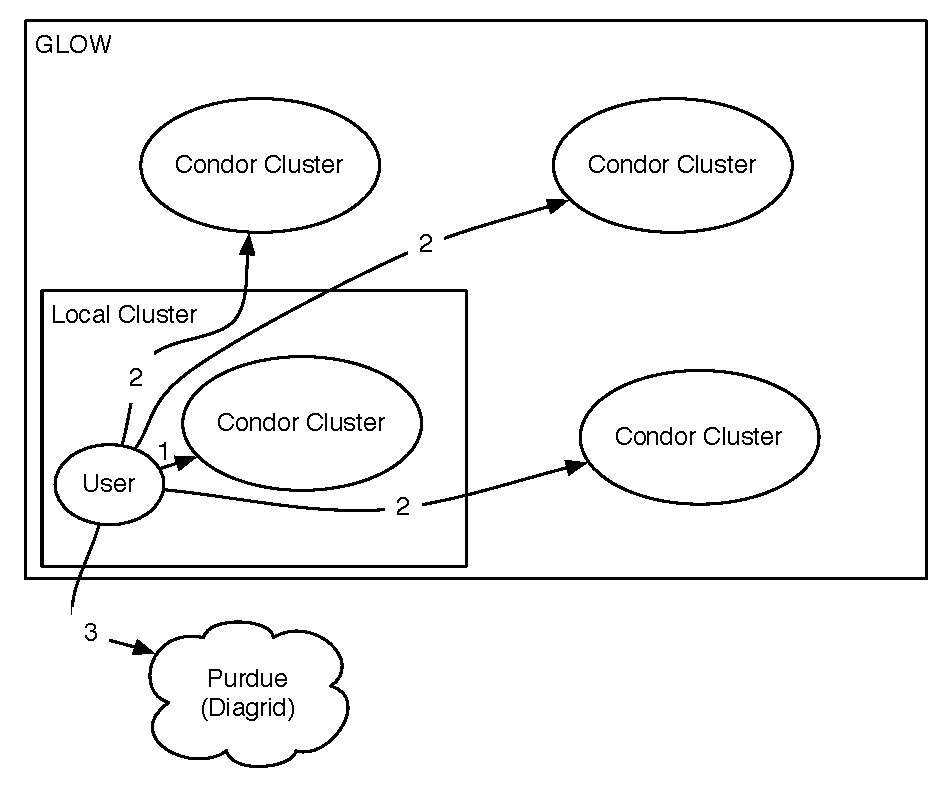
\includegraphics[scale=0.6]{images/GLOW-Campus}
\caption{Grid Laboratory of Wisconsin Campus Grid}
\label{fig:GLOWCampus}
\end{figure}


The Grid Laboratory of Wisconsin (GLOW) \cite{gridworkshopweb, glowwebsite} is a grid at the University of Wisconsin at Madison.  GLOW uses Condor to distribute 
jobs on their campus grid.  A diagram of the campus grid is shown in Figure \ref{fig:GLOWCampus}.  Security is based on IP whitelisting.  Since all resources are based on Condor, job 
submission and distribution is managed through the same Condor-only mechanisms as Purdue.  While there is a central 
team available to assist with management, each resource is free to define its own policies and priorities for local 
and remote usage.  Cluster ownership is distributed, although there's also a general-purpose cluster available.  
Software and data are managed by an Andrew File System (AFS) \cite{morris1986andrew} installation and Condor file transfer.  AFS is a global file system
that every worker node will mount, therefore providing a global space to store data and applications.  This simplifies data distribution
by providing a staging area.



\subsection{FermiGrid}
FermiGrid \cite{gridworkshopweb, chadwick2008FermiGrid} is made up of resources located at the Fermi National 
Accelerator Laboratory in Batavia, Illinois.  The FermiGrid campus grid is the closest example found of a ``mini-OSG".  Its 
uses the same Compute element software, information systems, and storage elements as the OSG.  Trust relationships on FermiGrid are 
based on the Grid Security Infrastructure (GSI) \cite{farrell2002rfc3281}, the same authentication method used by 
OSG.  Job submission is managed by Condor-G through a Globus submission layer to the clusters.  As this is the  same method  
used to submit to the OSG, it provides one strategy to getting users from campus to the national grid.  Most clusters are 
managed by a central team, while at least one is independently managed.  Some of the grid services (authorization and 
information services, for example) are run centrally.  Accounting is done through Gratia \cite{gratiaweb}, the same 
software that is 
used on the OSG.  A central cluster file system is available to most clusters, but Globus-based GridFTP file transfer is also 
heavily used.


%\begin{table}[h!t]
%\centering
%\footnotesize 
% Grid & Auth & Accounting & Storage & Submission
%\begin{tabular}{ | l | | l | c | c | c | c | c | c | c | }
%\hline
% & & Virginia & Oxford & Purdue & GLOW & FermiGrid & OSG \\
%\hline
%\multirow{4}{*}{Trust Relationships} & LDAP & \Checkmark &  & & & & \\ 
%\cline{2-8}
%& PKI & \Checkmark & \Checkmark & &  & \Checkmark & \Checkmark\\ 
%\cline{2-8}
%& Kerberos & & \Checkmark & & & & \\
%\cline{2-8}
%& Host & & & \Checkmark & \Checkmark & & \\
%\hline

%\end{tabular}
%\end{table}

\subsection{Overview of Campus Grids}
Table \ref{tab:campusgridoverview} compares the campus grid architectures with that of the OSG.  


\begin{table}[h!t]
\centering
\small
\begin{tabular}{ | p{50pt} | | p{68pt} | p{54pt} | p{60pt} | p{50pt} | p{60pt} |}
\hline
Grid & Trust & Job & Resource & Accounting & Data \\ 
& Relationship & Submission & Independence & & Management \\
\hline \hline
Virginia &  LDAP/PKI  & None \mbox{Described} & Strict & Central & None     \\ \hline
Oxford & Kerberos/PKI & Central & Central \mbox{Submission} & Custom & SRB  \\ \hline
Purdue & Host &  Distributed & Strict & Custom & Condor Transfer  \\ \hline
GLOW &  Host & Distributed & Strict & None &  Condor Transfer \\ \hline
FermiGrid & PKI & Central & Strict & OSG \mbox{Gratia} & Central File System  \\ \hline
OSG & PKI  & Distributed & Strict & OSG \mbox{Gratia} & Distributed \\ \hline
\end{tabular}
\caption{Campus Grid Attributes} \label{tab:campusgridoverview}
\end{table}



%\item 
%Many times no one has solved your exact problem before, but others have solved
%closely related problems or problems with aspects that are strongly analogous
%to aspects of your problem



\chapter{Design and Implementation of the HCC Campus Grid}
\label{sec:Implementation}

%\subsubsection*{What we (will do $|$ did): {\em Our Solution}}
%\begin{itemize}

%\item   Another way to look at this section is as a paper, within a paper,
%describing your implementation. That viewpoint makes this the introduction to
%the subordinate paper, which should describe the overall structure of your
%implementation and how it is designed to address the problem effectively.

%\item   Then, describe the structure of the rest of this section, and what each
%subsection describes.

%\item
%Created a campus grid integrating 3 clusters on a campus into a grid.  Submission to any of the clusters could overflow to the other 2.

%\item
%Overflow to the grid

%\item
%Using offline ads to efficiently match jobs to glideins on the non-condor cluster.

%\end{itemize}



%\subsubsection*{How our solution (will $|$ does) work}
%\begin{itemize}
%\item   This is the body of the subordinate paper describing your solution. It
%may be divided into several subsections as required by the nature of your
%implementation.

%\item   The level of detail about how the solution works is determined by what
%is appropriate to the type of paper (conference, journal, technical report)

%\item   This section can be fairly short for conference papers, fairly long for
%journal papers, or {\em quite} long in technical reports. It all depends on the
%purpose of the paper and the target audience

%\item   Proposals are necessarily a good deal more vague in this section since
%you have to convince someone you know enough to have a good chance of building
%a solution, but that you have not {\em already} done so.

The design of the Campus Grid at HCC attempts to meet these three goals:
\begin{enumerate}
\label{lst:hccgoals}
%\renewcommand{\labelenumi}{\textbf{Goal \arabic{enumi}} -- }
\item \textbf{Encompassing}: The campus grid should reach all clusters managed by HCC.
\item \textbf{Transparent}:  There should be an identical user interface for all resources, whether 
running locally or remotely.
\item \textbf{Decentralized}: A user should be able to utilize his local resource even if it becomes disconnected from 
the rest of the campus.  An error on a given cluster should only affect that cluster.
\end{enumerate}

\begin{figure}[ht]
\centering
\scalegraphics{images/HardwareOverview}
\caption{Overview of the Campus Grid hardware}
\label{fig:hardwareoverview}
\end{figure}

The campus grid framework is shown in Figure \ref{fig:hardwareoverview}.  The campus grid is made of user submission hosts, and resources.  The components of the campus grid are described in the next sections.

Along with these goals, the technologies in this chapter can be characterized by the framework described in Section \ref{sec:attributes}: trust relationships, job submission, resource independence, accounting, and data management.

\section{Campus Grid Factory} \label{sec:cgf}
To address the encompassing goal described above, the CGF was designed to bridge non-Condor clusters (\secref{sec:blahp}) into the campus grid. The CGF fulfills the decentralization, and resource independence, goal by attaching directly to a single cluster that it is serving, eliminating a central service.    

The Campus Grid Factory (CGF) is a collection of daemons that run on non-Condor clusters in order to submit pilots (\secref{sec:glideins}) when additional resources are requested.  The CGF includes a custom daemon, \texttt{campus\_factory} that is a wrapper around Condor, using functionality in Condor to talk to user queues and submit to the local resource manager.  The CGF instance must be on a `gateway' node in order to flock (\secref{sec:flocking}) with campus resources; the node must be able to talk to both the remote clusters and the local nodes.  The \texttt{campus\_factory} communicates with the \texttt{condor\_collector} daemon in order to detect requests for resources, and the \texttt{condor\_schedd} daemon to submit jobs to the Local Resource Manager (LRM).  




\begin{figure}[ht]
\centering
\scalegraphics{images/CGF-Close}
\caption{Overview of Campus Factory components}
\label{fig:cgfcomponents}
\end{figure}

The components of the Campus Grid Factory are shown in Figure \ref{fig:cgfcomponents}.  The CGF runs as a condor job on the local submission machine.  The CGF will communicate with remote queues, querying for idle jobs.  When idle jobs are detected, the \texttt{campus\_factory} will submit jobs as grid universe \texttt{PBS}.  The GridManager will handle interaction between the CGF's \texttt{condor\_schedd} and the BLAHP, which will translate the jobs to PBS submission syntax.  The \texttt{condor\_negotiator} and \texttt{condor\_collector} will communicate with remote queues.  The \texttt{condor\_collector} will maintain a list of active pilot jobs inside the cluster. 


\begin{figure}[ht]
\centering
\scalegraphics{images/CHEP-CGF}
\caption{Overview of Campus Factory Function}
\label{fig:cgf}
\end{figure}

The Campus Grid Factory functions are shown in Figure \ref{fig:cgf}. The CGF software starts by querying all 
the Condor schedds listed in a configuration file to determine if they have jobs to run (1).  If idle jobs are found, the \texttt{campus\_factory} will 
submit (2) a pilot job for execution to the PBS scheduler.  When PBS resources are available, PBS will start the pilot 
job (3) on an execute host, which becomes a Condor worker node.  After starting, the Condor worker node will contact (4) the 
Condor installation at the CGF and list itself as a node available to run jobs.  This is the ``pilot launch" sequence.

To launch user jobs, the CGF uses Condor flocking mechanisms.  The user schedd will first advertise (5) it is has idle jobs to run on the CGF's Condor collector.  
The CGF Condor negotiator matches the resources and orchestrates a direct connection (6) between the execute and 
submit hosts.  Then the execute host will transfer files and begin running the user job.

The CGF is an integral part of the campus grid because it allows non-Condor clusters to participate in the grid.  A Condor cluster would not need the CGF as it already can flock.  The CGF obeys the priorities set in the LRM allowing resource independence.  The CGF collector then is able to route jobs from other clusters to these available Condor job slots just as it would for an all-Condor cluster.

There are many architectural similarities between the CGF and GlideinWMS software: Condor pilot jobs, submission using a translation layer, and querying user queues to detect idle jobs.  However, GlideinWMS was not 
used since GlideinWMS is designed to have one central factory and a frontend on each submit host.
If a non-Condor cluster becomes disconnected from the GlideinWMS factory, even jobs that are submitted to a local cluster will 
be unable to run.  The GlideinWMS factory needs access to the cluster in order to start jobs, breaking the decentralization goal.  The 
CGF merges the roles of the frontend and factory in the GlideinWMS architecture, removing configuration and maintenance of a separate GlideinWMS daemon on the submit host. 
GlideinWMS is designed around GSI for security; while HCC uses GSI security for its OSG work, 
it is preferable to avoid making it a requirement for users running on the campus grid.

The GlideinWMS system prepares and validates runtime environments via a VO-supplied script, an 
essential element for removing a common source of grid frustration.  However, the runtime environment 
problem is lessened on campuses because of the smaller number of resources and the closer working relationships 
between system administrators.  It is unsolved at the inter-campus level.

Since the \texttt{campus\_factory} runs as a Condor job, the Condor daemons will ensure that it stays alive, eliminating the need to monitor an additional daemon.  

The \texttt{campus\_factory} depends on Condor daemons to carry out many tasks such as:
\begin{itemize}
\item Run and maintain the \texttt{campus\_factory} daemon.
\item Submit the pilot jobs to the LRM (See Section \ref{sec:condorandblahp}).
\item Collect and advertise information on the pilot jobs.
\item Negotiate with submitters in order to route jobs to the pilots.
\end{itemize}



\subsection{Flocking} \label{sec:flocking}

In the GLOW and Purdue campus grids, every resource runs the same scheduler, Condor.  They use Condor's Flocking mechanisms to distribute jobs between clusters.

Flocking \cite{epema1996worldwide} is a method of linking Condor clusters into a larger grid.  Flocking was illustrated in Figure \ref{fig:Flocking}.  Condor daemons are described in Table \ref{table:condordaemons}.  When a user submits jobs to Condor, they are stored and managed by the \texttt{condor\_schedd}.  The \texttt{condor\_schedd} acts as an agent on the user's behalf to keep track of jobs, and place jobs efficiently.  Flocking improves the job submission and transparent execution environment of campus grid jobs by eliminating the need to explicitly specify pools for execution.  It improves data management by directly transferring files from the submitter to the execute host, bypassing the gatekeeper.  Job file dependencies are described in the submission file.  Typically in the OSG, job data is staged to the gatekeeper or a storage element before transferring to the worker node.  Condor will handle faults in flocked jobs, such as resources going away and disconnections to remote resources, just as it would a local job, leading to better decentralization of the campus grid.

After the jobs have been submitted, the \texttt{condor\_schedd} will maintain an integer \texttt{FlockLevel}.  At first, the \texttt{FlockLevel} will be set to 0 and jobs will only run on the local resources.  After a few minutes, if there are still idle jobs in the queue, the \texttt{FlockLevel} will increase by 1.  Each time the \texttt{FlockLevel} increases, the \texttt{condor\_schedd} will advertise to another Condor pool in the flocking list that it has idle jobs to run.  When the remote Condor pools see idle jobs, the \texttt{condor\_negotiator} for that pool will contact the \texttt{condor\_schedd} to attempt to match jobs to the remote resources.    If a match is found, the schedd directly contacts the execute host to begin running the job.  

Flocking does not delegate responsibility for a job.  The original \texttt{condor\_schedd} will maintain the job, transferring input and output and monitoring its status.  This is analogous to hub-and-spokes: the job ownership never moves, but the jobs can execute at multiple resources.

The CGF uses flocking for job distribution.  The CGF will flock jobs to and from other campus resources.


\subsection{Condor \& BLAHP} \label{sec:blahp}
\label{sec:condorandblahp}

If the grid does not have the same scheduler on all clusters, there needs to be a translation layer from one scheduler to another.  The Batch system Local ASCII Helper Protocol (BLAHP) was designed to offer a simple abstraction layer over different local resource manager services, providing uniform access to the underlying computing resources \cite{blahp}. BLAHP is maintained by the gLite \cite{glite} collaboration at the European Organization for Nuclear Research (CERN).  The BLAHP supplements the encompassing goal by allowing execution of Condor jobs to the underlying resource manager.  

BLAHP is distributed with Condor as an additional library.  Condor uses BLAHP to submit jobs when specifying the PBS or LSF \texttt{universe} in the submission file.  

BLAHP is used by the CGF to submit pilot jobs to the underlying batch system.  The \texttt{campus\_factory} only needs to communicate with Condor in order to submit to the underlying PBS scheduler.


\subsection{Pilot Jobs} \label{sec:glideins}
Condor Glidein \cite{frey2002condor} is a pilot job--based grid submission that creates an overlay network on remote resources.  Glidein uses the pilot method for job execution.  When a Glidein starts, it advertises its availability to run jobs.   Glidein is designed to use standard Condor mechanisms to advertise its availablity to a Condor Collector process, which is queried by the Scheduler to learn about available resources.  Each user job running in a glidein is run in a sandbox on the local disk and is provided with a consistent execution environment across hosts and clusters.

\begin{figure}[ht]
\centering
\scalegraphics{images/LayeredDiagram}
\caption{Layered Diagram of the Worker Node}
\label{fig:wnlayereddiagram}
\end{figure}


The worker node layered diagram is shown in Figure \ref{fig:wnlayereddiagram}.  In the figure, you can see that the hardware and OS are the same for both PBS and Condor clusters.  But, since PBS is the native scheduler on a PBS worker node, abstractions must be built on top of it.  The Glidein Wrapper is a script I developed to create the glidein sandbox, and start the glidein daemons.  This creates a single interface to Condor\_Startd's, regardless of which cluster the user is communicating with.  

Pilot jobs are used by many physics experiments \cite{nilsson2008experience, zvada2010cdf, bradley2010use}.  Physics experiments create pilot frameworks because they want a consistent execution environment across hundreds of clusters.  Pilot workflow management systems have the following benefits.
\begin{itemize}
\item \textbf{Scheduling Optimization:} The pilot reports only when a CPU is immediately available to run a job.  This is in contrast to direct submission to a grid resource, where after submission, you have committed to running on that resource.  If idle cores become available on another cluster, you are unable to execute on them as long as your job is submitted elsewhere.  
\item \textbf{Input/Output Automation:} The pilot can transfer input and output for the user directly to the worker node.  This bypasses a possible bottleneck at the grid gatekeeper.  Additionally, the pilot can be customized to transfer input from third parties such as storage elements.
\item \textbf{Monitoring:} The monitoring of a job is improved by the pilot infrastructure.  The grid translation layers between the local batch system and the grid interface can hide many errors and incorrectly report usage.
\item \textbf{Fault Tolerance:} A job failure can be more accurately detected and recovered inside the pilot.  The pilot can detect that the payload job has failed and report back the error.  Additionally, it can verify the environment is acceptable for jobs before allowing jobs to begin.
\item \textbf{Multiple Runs:} Each pilot can run multiple jobs serially, reducing submissions through the site gatekeeper.  This will increase throughput since only a single authentication is necessary between the pilot and the user.
\end{itemize} 

Condor Glidein jobs require several condor daemons packaged with a wrapper script.  When the job starts, the Glidein job will:

\begin{enumerate}
\item Create a temporary directory on the local disk.  This will be used for the job sandboxes.
\item Unpack the glidein executables onto the local disk.
\item Set the late binding environment variables for Condor to point to the temporary directory.
\item Start the  \texttt{condor\_master} daemon included in the glidein executables.
\end{enumerate}

The \texttt{condor\_master} will start the \texttt{condor\_startd} daemon which will advertise itself to the glidein collector, making the node available for remote jobs.  

Glideins are being used in production in the Open Science Grid using the software GlideinWMS \cite{sfiligoi2008glideinwms}.  
%They provide several advantages over regular job submission.  Each glidein sandboxes and monitors the user jobs it runs.  The glidein can run multiple user jobs inside a single LRM job and will continue to run until the configured time to stop.  



\subsection{Pilot Submission Algorithms }
The \texttt{campus\_factory} process decides whether to submit pilots to the underlying non-condor cluster.  The  \texttt{campus\_factory} has two configuration options relating to submission of pilots to the LRM: \texttt{MaxIdleGlideins} and \texttt{MaxQueuedJobs}.

\begin{description}
\item[ \texttt{MaxIdleGlideins}] \hfill \\
An integer representing the number of idle slots that will be allowed before the  \texttt{campus\_factory} stops submitting jobs. 

\item[ \texttt{MaxQueuedJobs}] \hfill \\
The maximum number of queued pilots that will be idle in the queue of the LRM. 

\end{description}

The  \texttt{campus\_factory} will query user queues and record the number of idle jobs.  When there are idle jobs at user queues, it will use the following logic to determine how many pilot jobs to submit.  The variable \texttt{idleuserjobs} in Algorithm \ref{alg:glideins} are the recorded number of idle jobs at user queues.

The  \texttt{campus\_factory} submission logic is as follows:

\begin{algorithm}
\begin{algorithmic}
\STATE $idleuserjobs \gets$ QueryUserQueues()
\IF {idlejobs $<$ MaxIdleGlideins \&\& queuedglideins $<$ MaxQueuedJobs}
	\STATE $toSubmit \gets$ min(MaxIdleGlideins - idlejobs, MaxQueuedJobs - queuedglideins, idleuserjobs)
\ELSE
	\STATE $toSubmit \gets 0$
\ENDIF
\RETURN $toSubmit$

\end{algorithmic}
\caption{Algorithim for determining how many pilots to submit.}
\label{alg:glideins}
\end{algorithm}

Note that the QueryUserQueues function requires the \texttt{campus\_factory} to implement external communication with the user queues.

Additionally, the  \texttt{campus\_factory} has logic to detect pilots that are not reporting to the collector.  Pilots that have been submitted to the CGF's Condor instance will show their status as reported by PBS and BLAHP.  The \texttt{campus\_factory} will look for the same number reporting as `Running', and reporting to \texttt{condor\_collector}.  If these two numbers differ by more than $10$ percent, the \texttt{campus\_factory} will stop submitting jobs.  This can happen when the LRM cannot transfer files, if the BLAHP is incorrectly reporting the status of a job, or if there is something wrong with the pilot jobs.


\subsection{OfflineAds} \label{sec:offlineads}
OfflineAds are a Condor feature that were designed to be used for power management.  When a node hasn't been matched for a configurable amount of time, the machine can be turned off to save power. When the machine is preparing to turn off, it sends an OfflineAd to the collector that describes the machine so that it can be restarted if needed.  OfflineAds are in the HCC Campus Grid used to optimize the submission of pilot jobs to the underlying batch system.   
  The OfflineAd is just a normal ClassAd that includes all of the features that can be used when matching against an online resource, such as memory, disk space, and installed software.  When the OfflineAds describing the machine are matched to a job by the Condor negotiator, the negotiator inserts a new attribute into the OfflineAd called \texttt{MachineLastMatchTime}.  When used for power management, the Condor Rooster daemon periodically queries the collector for the OfflineAds.  If one has been recently matched, then it wakes the corresponding node.

%The collector maintains the offline ads for a configurable amount of time using the configuration variable OFFLINE\_EXPIRE\_ADS\_AFTER. During this time, 

In the \texttt{campus\_factory}'s implementation, the OfflineAds are used to match possible pilot resources to idle jobs.  Dead pilots are thought of as ``offline machines.''  Again, the \texttt{condor\_negotiator} will treat the OfflineAds just as it would a real ad and matches it to idle jobs.  Since the OfflineAd is an exact copy of a running glidein, it is reasonably expected that one can get a similar glidein when you submit to the local scheduler.  As the negotiator sees no difference between running and OfflineAds, the OfflineAds will be matched even when flocking from another Condor pool.

Since the OfflineAds are exact copies of previously live pilots, the OfflineAds increase the accuracy of matching with idle jobs by exactly resembling running glideins.  In GlideinWMS and previous pilot implementations, filters were applied to the user queues to determine if a job was capable of running on the resource.  The filters were customized by administrators to route jobs to the pilots that matched their requirements.


\subsubsection{Influence OfflineAds Have on the CGF}
The OfflineAds do not completely replace all the logic described in Algorithm \ref{alg:glideins}. The site must still meet the idle glideins and idle slots requirements that were originally used to throttle new pilot submissions. The OfflineAds replace the need for the \texttt{campus\_factory} to query remote schedds for idle jobs.  This improves the efficiency and simplicity of the \texttt{campus\_factory} by eliminating communication.  But the large benefit is the increased accuracy of the pilot descriptions.  The \texttt{campus\_factory} will only submit jobs when the OfflineAds detect a definite match to the cluster's resources.  The negotiator and collector take care of all job matching with accurate glidein ClassAds.

The logic of the \texttt{campus\_factory} is described in Algorithm \ref{alg:glideinswithofflineads}. 


\begin{algorithm}
\begin{algorithmic}
\STATE $idleuserjobs \gets$ QueryOfflineAds()
\IF {idlejobs $<$ MaxIdleGlideins \&\& queuedglideins $<$ MaxQueuedJobs}
	\STATE $toSubmit \gets$ min(MaxIdleGlideins - idlejobs, MaxQueuedJobs - queuedglideins, idleuserjobs)
\ELSE
	\STATE $toSubmit \gets 0$
\ENDIF
\RETURN $toSubmit$

\end{algorithmic}
\caption{Algorithim for determining how many glideins to submit with \mbox{OfflineAds}}
\label{alg:glideinswithofflineads}
\end{algorithm}

In contrast to Algorithm \ref{alg:glideins}, this does not have any external communication.  The QueryOfflineAds queries the local \texttt{condor\_collector}.

\subsubsection{Creating OfflineAds}
After the \texttt{campus\_factory} submits pilot jobs, it detects the classads of running pilot jobs, copies the classads, and re-advertises them as OfflineAds. 

The changes required to transform a glidein classad into an OfflineAd are listed in Table \ref{tab:offlineads}. 

\begin{table}[h!t]
\centering
\begin{tabular}{| l | l | p{6cm} |}
\hline
ClassAd & New Value & Comment\\ \hline \hline
Offline & True & Enable the OfflineAd logic in Condor daemons.\\ \hline
Name & Unique name & Mandatory name for indexing in the Condor collector.\\ \hline
MyCurrentTime & LastHeardFrom - Time now & Used for offset time.   \\ \hline
ClassAdLifetime & 24 hours & To address a bug in the handling of OfflineAds by Condor. This is how many seconds the collector will keep this ad. \\ \hline
State & Unclaimed & Make sure it will match with idle jobs. \\ \hline
Activity & Idle & Again, for matching  \\ \hline
PreviousName & Name & Value of 'Name' attribute of the original ad. Useful for debugging. \\ \hline
\end{tabular}
\caption{Changes to ClassAds for Offline Function} \label{tab:offlineads}
\end{table}



\subsubsection{Managing OfflineAds}
By default, the factory will attempt to maintain a specific number of OfflineAds. By default, it maintains the newest 10 ads.  One can sort by different `types' of machines (big memory, big disk), and keep an assortment of unique ads.  This method will better represent the heterogeneous nature of the resource.  Ten was determined to be an appropriate sample size as it is large enough to represent multiple nodes (currently eight cores per node standard).  Larger number of ads will cause a heavier load on the CGF as it matches the OfflineAds to idle jobs.

The factory will maintain the newest 10 OfflineAds.  If it detects less than ten, the OfflineAd manager will list the site as delinquent in an internal structure and will recommend the factory submit more pilots to the LRM.





\section{Bridging Campus Grids} \label{sec:bridging}
There are two methods for expanding the campus grid: through GlideinWMS to the OSG, 
or by bridging campuses through flocking.  Bridging provides a method for jobs to leave the boundaries of the campus. The benefits of bridging externally are obvious--increased throughput 
for the local user's jobs.  HCC has been able to  
bridge to the GLOW, Purdue, and FermiGrid grids discussed in Section \ref{sec:others}.  We connect to FermiGrid and GLOW through the OSG and 
to Purdue via Condor flocking.

Unlike the OSG, where the trust relationship is defined by a central consortium and agreed upon by all sites, trust is established between 
campuses with flocking on a case-by-case basis.
The current model for trust is based on limited trusted hosts (IP based authorization).  Each site publishes a list of submit and negotiator 
hosts that are trusted to submit and accept jobs, respectively.  This implicitly trusts an entire campus, while the OSG 
trust model is based on virtual organizations that may have no relationship to a physical campus or submit host.

\begin{figure}[h!tbp]
\begin{center}
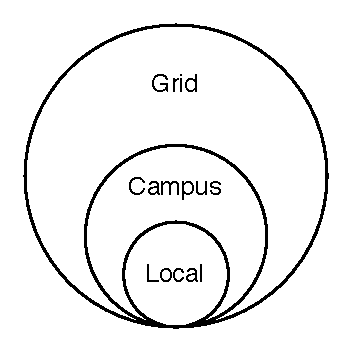
\includegraphics[scale=0.8]{images/BWCircles}
\caption{Widening Circle of Resources}
\label{fig:circleresources}
\end{center}
\end{figure}

The ever-widening circle of resources expands from the locality of the user (Figure \ref{fig:circleresources}).  It goes from the resource 
the user knows best (and has the best support for), the local cluster, to the most foreign one, the national grid.  This is a very natural progression. 
Each step described comes with more complexity and new failure modes.  If the user is ever frustrated at one 
transition, he can just remain contented with the resources he has, as opposed to having to switch between ``local 
mode" and ``grid mode," as must be done with Condor vs Condor-G.  Another usability advantage is that all end-user interfaces are Condor.  The user 
never encounters errors translated between systems (a common user frustration); the user needs to develop expertise 
in Condor alone.


\section{Full Campus Infrastructure} \label{sec:fullcampus}

\begin{figure}[h!tbp]
\begin{center}
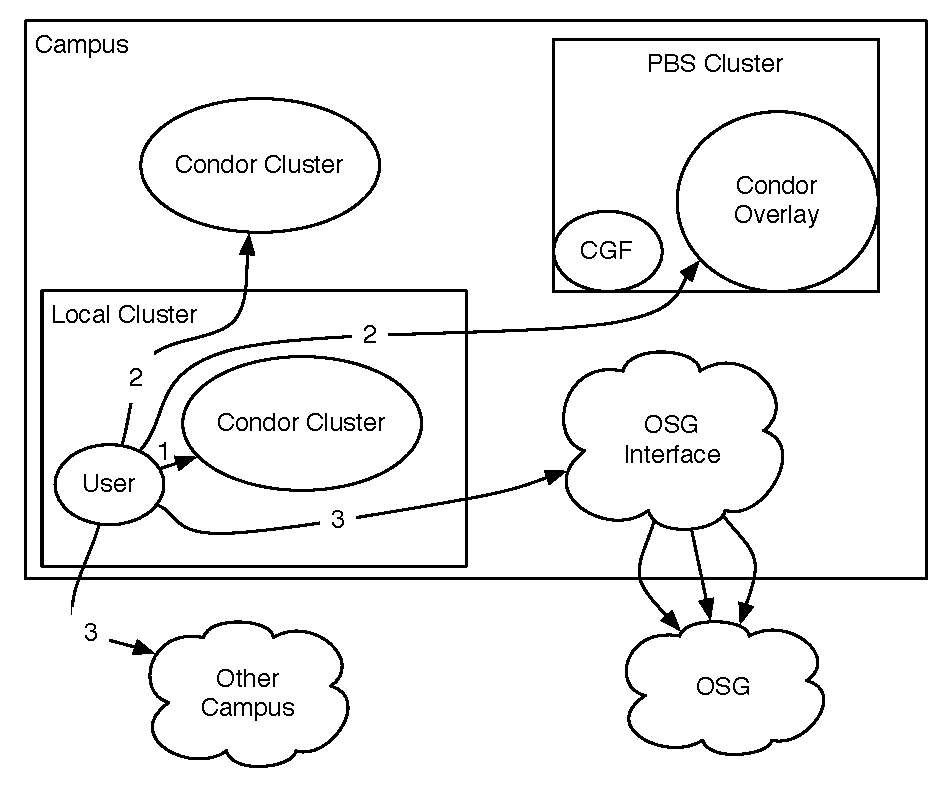
\includegraphics[scale=0.8]{images/CHEP-Campus}
\caption{The Full Campus Grid Architecture}
\label{fig:campusgrid}
\end{center}
\end{figure}

The full campus grid architecture with bridging is shown in Figure \ref{fig:campusgrid}.  This campus infrastructure includes all the on-campus resources, as well as meets the goals of the campus grid: Encompassing, Transparent, and Decentralized.
The 
user first submits jobs to the local Condor cluster (1).  If the local cluster can fulfill the user's needs, then all the 
jobs will remain there.  If the local cluster is full or cannot meet the user's demand, Condor flocking will start 
jobs on other campus clusters (2), either with pure Condor or utilizing the CGF.  If the on-campus 
resources are unable to meet the user's request, the local Condor schedd will expand its reach again (3) by looking 
outside the campus.  The jobs can also be sent to the OSG via flocking to a GlideinWMS 
frontend, which creates an overlay pool of grid resources.  In this architecture, every effort is given to find 
resources for the user (local, across campus, or across the nation), while maintaining the same Condor interface for the user.

\begin{figure}[ht]
\centering
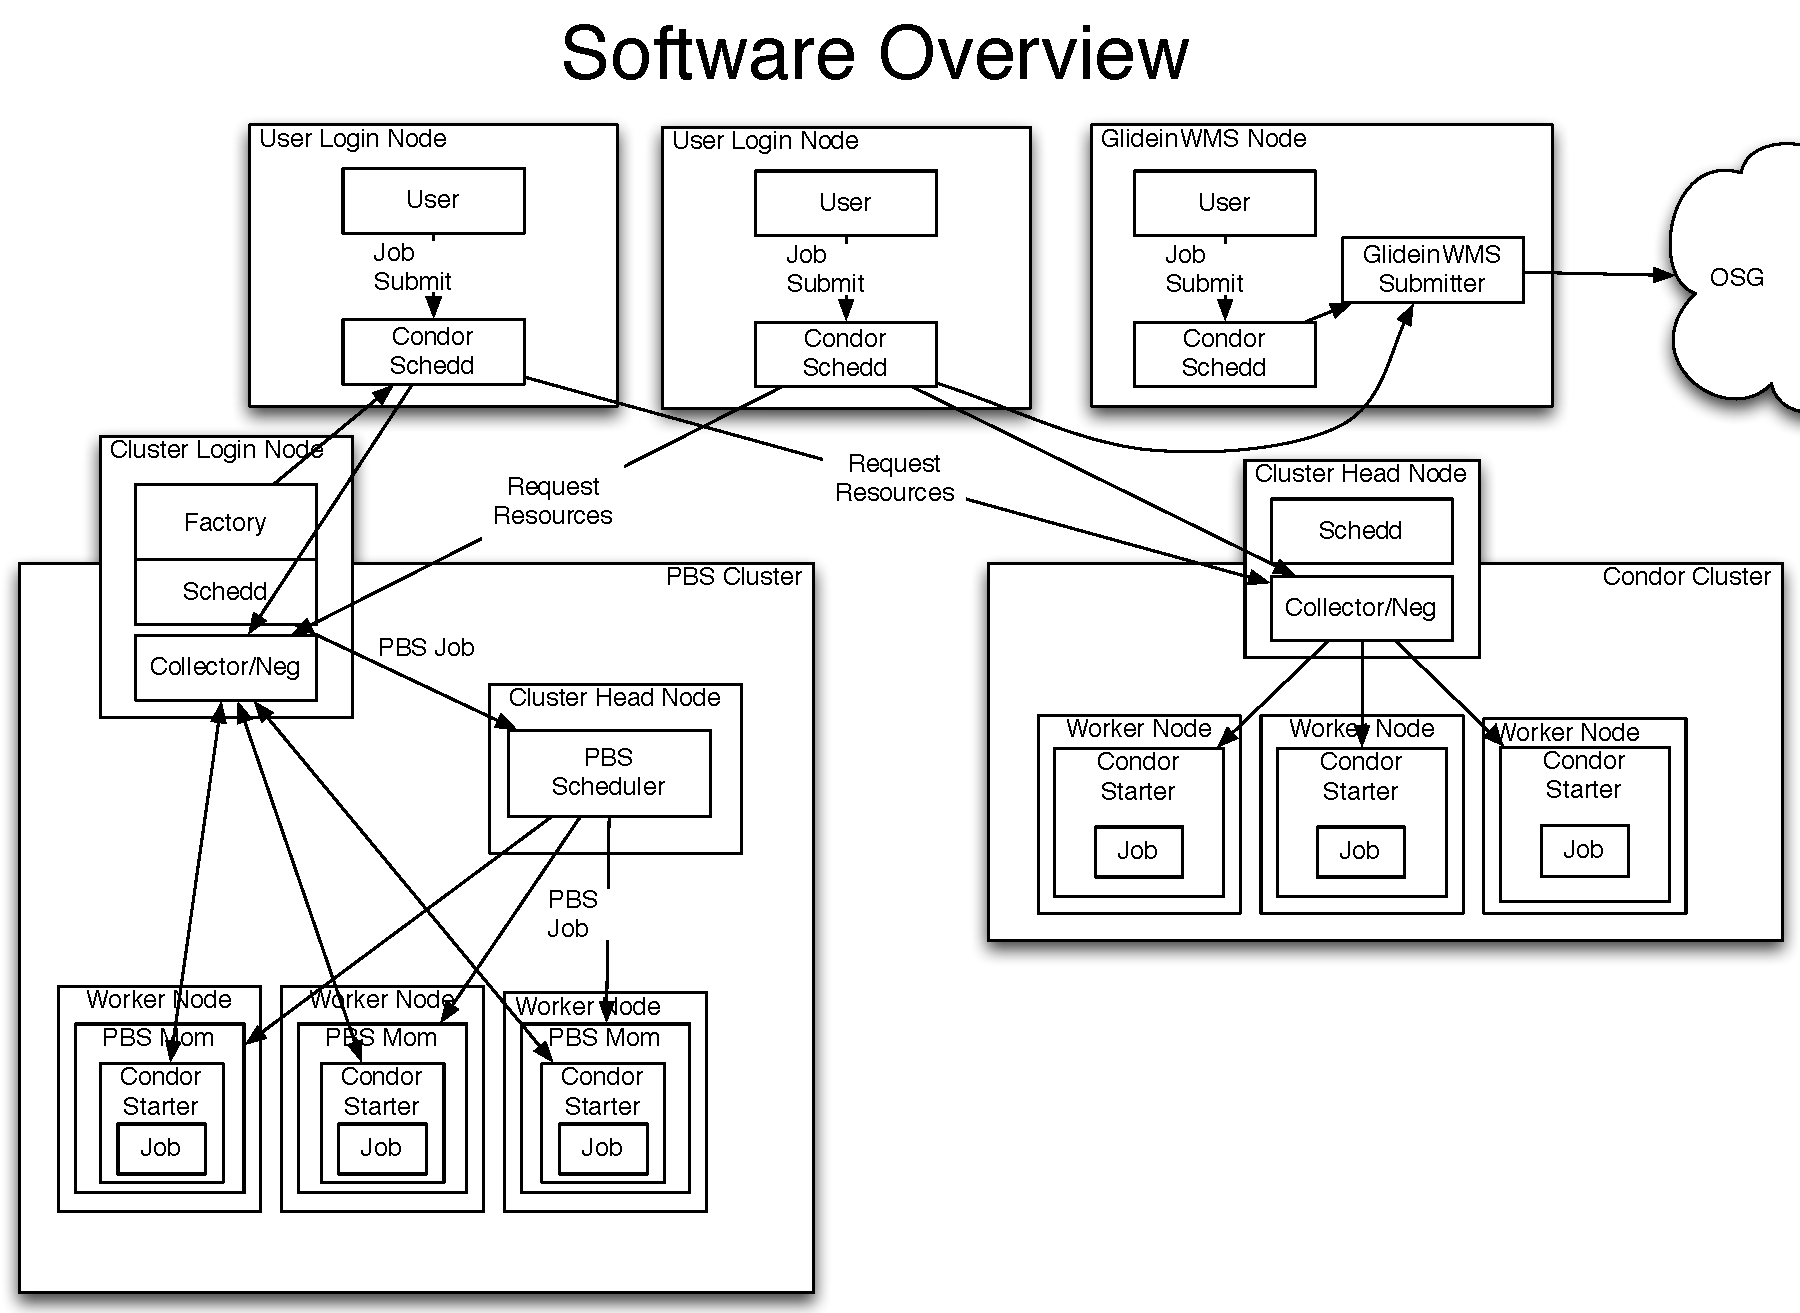
\includegraphics[angle=90, scale=0.6]{images/SoftwareOverview}
\caption{Overview of the Campus Grid software}
\label{fig:softwareoverview}
\end{figure}

The software described in the previous sections are further shown in Figure \ref{fig:softwareoverview}.


%\textbf{ Campus Factory is the heart of the operation.  It provides all throttling and logic to the submit of glidein jobs to the non-condor cluster.}
















\chapter{Evaluation}
\label{sec:Evaluation}

%\section{Experimental Setup}

This chapter is divided into two sections, details of the HCC Campus Grid in \secref{sec:hcc}, and evaluation and comparison of the HCC Campus Grid in \secref{sec:evaluationcharacteristics}.

\section{University of Nebraska Holland Computing Center Campus Grid} \label{sec:hcc}

In order to evaluate the framework described in this thesis, a campus grid was implemented at the Holland Computing Center (HCC).  A diagram describing the HCC Campus Grid is shown in Figure \ref{fig:hccgrid}.  In this diagram the user submits jobs on a central machine.  First, the jobs will attempt to run on campus resources at the clusters Prairiefire and Firefly.  Next, it will branch out to the GlideinWMS interface and flocking to Purdue.

\begin{figure}[h!tb]
\begin{center}
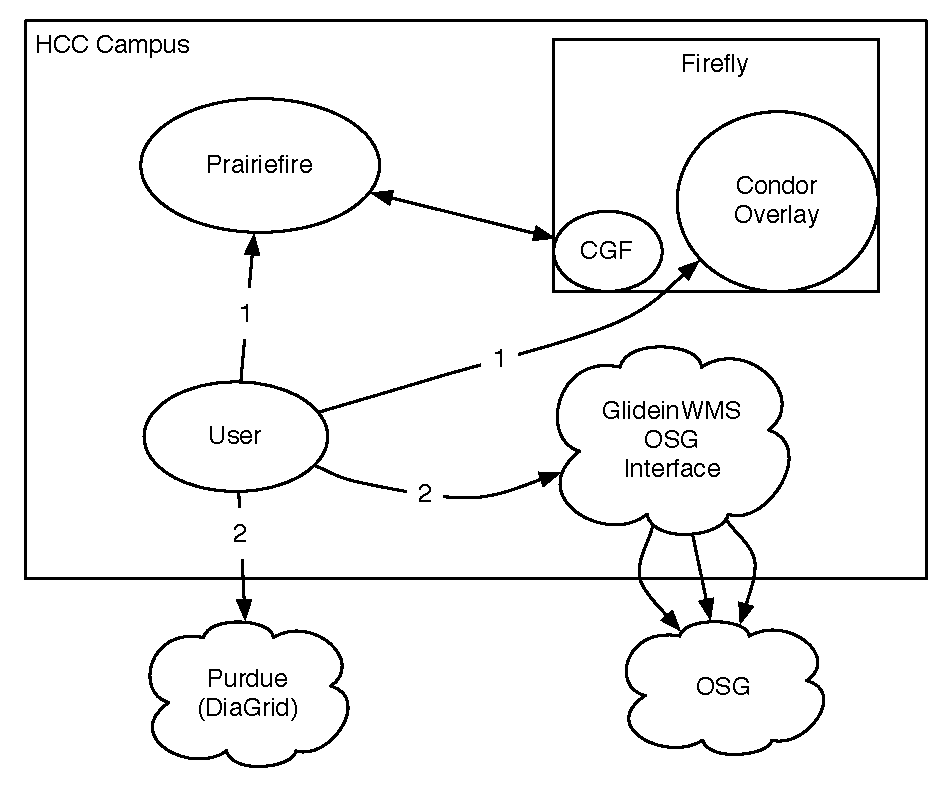
\includegraphics[scale=0.8]{images/HCC-CampusGrid-012411}
\caption{The HCC Campus Grid}
\label{fig:hccgrid}
\end{center}
\end{figure}


Like Purdue and GLOW, we have based the campus grid upon Condor and flocking.  Each resource has a Condor-based interface, giving an 
identical user experience regardless of what the user considers his or her ``local" cluster.  While one of the local 
clusters run Condor as the primary batch system, the other is based upon PBS.  PBS was chosen because of its ability to plan  
large-scale parallel jobs run on the resource.  GLOW's Condor-only approach did not fit our case due to the PBS requirement, and 
Purdue's model of running multiple schedulers was rejected because we wanted a less-invasive approach and because we 
wanted more efficient scheduling. The Campus Grid Factory (CGF)  
provides a Condor interface for our PBS cluster; as covered in Section \ref{sec:cgf}.

%To enable decentralized operation, we utilized Condor flocking \cite{epema1996worldwide} between clusters.  Condor 
%flocking enables a transparent execution environment on remote resources by 
%imitating local resources during the interaction between the submit and execute hosts.  The jobs will continue 
%to be managed by the original user's submit host, but the execute hosts can be outside what is managed by the local 
%Condor pool.  Furthermore, flocking can handle communication errors between remote hosts and can recover, 
%providing disconnected operation when resources are unreachable.

Through Condor flocking and the CGF, we have successfully encompassed all local resources.  To provide even more value 
to HCC, jobs can also bridge to the OSG and other campus grids.  The interface to the OSG uses the GlideinWMS \cite
{sfiligoi2008glideinwms, sfiligoi2008making} frontend software, while we link to other campuses using Condor flocking 
(the same method Purdue uses to link the campuses of DiaGrid).  Unlike Condor-G, which provides a Condor interface to 
GRAM, these two methods give the same user experience as using Condor as a batch system.

All clusters on the campus grid are managed by the Holland Computing Center; therefore, the trust relationship 
between the hosts are implicitly strong.  A special account is set aside on the PBS cluster for the CGF to run 
campus grid jobs.  The CGF daemon also runs as this user.  On the Condor-managed cluster, campus grid jobs run as user \texttt{nobody} while locally-submitted 
jobs run as the submitting user.

Because resources are run by the same organization, we have the ability to provide distinct user priorities per resource 
through Condor.  Further, because Condor runs \textit{inside} PBS rather than alongside it, PBS can schedule its jobs 
without interrupting Condor ones.  An administrator can prioritize jobs submitted directly from the local cluster over 
those from a remote submission, even for the same user.

Each submission host runs the Gratia accounting software to provide user accounting.  Gratia was chosen because of:
\begin{itemize}
\item Integration into the larger OSG accounting.
\item Separation between remote clusters and the central database (updates are done via HTTP).
\item Ability to integrate new resource types easily.

\end{itemize}  .  For integration in the OSG, 
we have extended the software to record both the submission host and the remote OSG cluster utilized.

HCC does not have a shared file system across all clusters, so the HCC Campus Grid data management is handled by Condor file 
transfer.

%\subsubsection*{Social political stuff}

%\subsubsection*{How we tested our solution}


The environment includes two local clusters, as well as an interface to the OSG and another campus grid.

\subsection{Prairiefire Cluster Configuration} \label{sec:prairiefiresetup}
Prairiefire is running both Condor and PBS in a side-by-side configuration.  This is very similar to how Purdue uses Condor.  When a PBS job arrives on a node, the Condor daemons will preempt the running job and move to another node.  Therefore, PBS has priority access to nodes, while Condor is treated as an opportunistic user.

Condor runs on the head node of the cluster.  The head node has both a public and private interface.  Each worker node connects to the outside world through a Network Address Translation (NAT) layer.  The NAT is used to aggregate the outside connectivity of the cluster by funneling traffic through a single gateway.  Since Condor must have direct communication between the submitter (possibly outside of Prairiefire) and the execute host (worker nodes), Prairiefire must run the Condor Connection Broker (CCB).  The CCB runs on the head node and negotiates connections for nodes behind the NAT to connect with the submitter.

Prairiefire will schedule jobs from the Firefly CGF and the GlideWMS submit machine to run via Condor flocking.  Prairiefire's head node can also flock jobs to Firefly.  These interactions are shown in Figure \ref{fig:hccgrid}.  To do this, the configuration variable \texttt{FLOCK\_FROM} was set to \texttt{ff-grid.unl.edu, glidein.unl.edu} and \texttt{FLOCK\_TO} to \texttt{ff-grid.unl.edu}.   Further, the security is set up such that jobs coming from outside of the Prairiefire pool will use the user \texttt{nobody} when running the job.  Condor uses this unprivileged account so that a rogue user can cause minimal impact to the system, and to protect other users of the system.  The security on the machine is IP based; it trusts all users from the \texttt{FLOCK\_TO} and \texttt{FLOCK\_FROM} hosts.




\subsection{Firefly Cluster Configuration}
Firefly is running the Campus Grid Factory (CGF) on a node straddling the border of the public and private networks.  Unlike the interactive login node, the CGF host does not have a firewall installed as Condor uses many ports. 

The CGF runs as a local unprivileged user.  Condor is installed in this user's home directory and runs under this user's account.  The CGF runs as a Condor job; it is maintained by the Condor schedd.  Submissions to PBS use the default queue.

The Condor instance that runs on the gatekeeper is configured to allow flocked jobs from Prairiefire and the GlideinWMS submission node.  Also, users can submit jobs to the CGF's Condor instance at Firefly, allowing them to run on Firefly or flock to Prairiefire.



\subsection{GlideinWMS OSG Interface Configuration}
The GldeinWMS interface runs the GlideinWMS frontend software, as well as a Condor installation.  The frontend periodically queries the queues of multiple campus machines to detect idle jobs.  When idle jobs are present, the frontend sends a request for glideins to be submitted to the GlideinWMS factory.  The HCC frontend requests glideins from the central OSG factory run at the University of California at San Diego.  

Glideins are submitted to resources across the country on behalf of HCC.  When the glidein jobs start on the remote resources, they pull Condor executables from the central factory, start them, and contact the HCC frontend to request jobs.


\subsection{Flocking to Purdue Configuration}
Flocking to Purdue is enabled by publishing a list of collectors and schedds at Purdue and HCC.  This list is then manually inserted into the configurations of machines that will send and receive jobs.  The collector locations are placed in \texttt{FLOCK\_TO} and the schedds are specified in \texttt{FLOCK\_FROM}.

Security between the hosts are established with the \texttt{CLAIMTOBE} environment in Condor.  In this environment, Condor trusts the daemons to give accurate information on job ownership and authentication.  The security is further refined by limiting the authentication to only the Collector and Schedd hosts specified above.  This is the same method used on the HCC campus grid described in \secref{sec:prairiefiresetup}.

In total, Purdue has seven collectors and six schedds participating in the flocking.  HCC has two collectors and three schedds.


\subsection{User Submission}
User submission is by design very similar to submission on a dedicated Condor resource.   The user will specify the executable and where to store the stdout and stderr.  Input files are transferred per-job to the execute machine.  Condor will automatically determine output files by scanning the sandbox directory for any new files created.  The new files will be transferred back to the submitter.

Condor will only transfer files when the variables \texttt{should\_transfer\_files} and \texttt{when\_to\_transfer\_output} are set.  A typical submission file is shown in Figure \ref{fig:submission}.  In the example, Condor will transfer the executable (\texttt{/bin/hostname}) to the execute host.  Condor will return the stdout and stderr from the execute host back to the submitter.

\begin{figure}[h!t]


\centering
\lstset{
backgroundcolor=\color{white},
showspaces=false,
basicstyle=\footnotesize}
\subfloat[Non-Campus Grid submission]{
\fbox{
\lstinputlisting[boxpos=b]{include/non-grid.txt}
} % fbox
} % subfloat

\hspace{10pt}

\subfloat[Campus grid submission]{
\fbox{
\lstinputlisting[boxpos=b]{include/grid.txt}
} % fbox
} % subfloat



\caption{Campus Grid Submission Scripts} \label{fig:submission}
\end{figure}


\section{Characteristics of HCC Campus Grid} \label{sec:evaluationcharacteristics}
This section evaluates the HCC Campus Grid on the characteristics defined in Section \ref{sec:attributes}.  

\subsection{Trust Relationships}
On most campuses, trust relationships are very strong.  On some campuses, a single group maintains the campus clusters.  On others, the proximity of administrators has facilitated trust.

At HCC, one group administers the clusters on campus, therefore the trust relationship is strong.  The execution gateways in the campus grid restrict access by IP address.  Therefore, there is a set of trusted submission hosts.  Each host trusts each other's claimed user authentication.   Additionally, jobs running on the CGF use a valid user account rather than a un-privileged account such as user \texttt{nobody}.

When we compare this to other campus grids, we can see that the IP based filtering policy is consistent with some campuses, and less restrictive than others.  

In the Virginia Campus Grid, the user uses LDAP and PKI for authentication.  The user first authenticates with local LDAP servers, then creates a PKI certificate to interact with the on--campus clusters.  While the LDAP authentication is consistent with on-campus policies, PKI is not.  The series of interactions complicates the authentication with the servers, and necessitated the creation of a separate daemon called CredEx.  The HCC policy requires only one authentication with a submit host to have access to the campus grid.

In the Oxford Campus Grid, Kerberos is used for on campus submissions, while PKI is used for external access.  This is consistent with on-campus policies.

The OSG focuses on the security of execution gateways (Compute Elements) as opposed to the security of submission hosts. Though a compromise of a gateway can lead to access of many short--lived, limited proxies, the compromise of a submission host can give access to a long--lived, unlimited proxy of a few users.  Further, since the OSG allows unregistered submission hosts, and they are relatively easy to set up compared to the gateways, there are many submission hosts.  OSG CE's most often maintained by professional or knowledgable administrators; in contrast, submission hosts may be maintained by users with limited knowledge of security.  Submission hosts could be compromised without knowledge of their owners, and could give access to unrestricted certificates.  Thus, we argue the whitelisting of submit hosts under the care of known, dependable system administrators outweigh the lack of ``strong security'' between submit hosts and resources.  

The GLOW and Purdue campus grids are similarly IP security based grids.  The IP based security simplifies the setup of a grid based on Condor flocking that GLOW, Purdue, and HCC use.  The submission host is additionally protected by the fact it only submits jobs to known good hosts.

The trust relationships inside campuses are simple compared to those outside of campus.  When jobs begin flowing outside the local domain, the authentication must match that of the external entity.  Jobs flow off campus through flocking to external campuses and to the OSG through the GlideinWMS interface.

When flocking to external campuses, the HCC grid again uses IP based security negotiated with the campuses.  In practice, this involves publishing a list of trusted hosts on each campus.  Since campuses usually use a single authentication method for all of their machines, this creates a scenario where either a campus will trust the entirety of another campus, or not at all.  For example, HCC trusts all of Purdue's submit hosts, and therefore all of the Purdue users.  More accurately, we trust the Purdue administrators  to monitor their users' usage, and to contain and contact us about possible security threats.

When jobs move to the OSG, we must match the authentication methods used on the OSG, which is PKI.  GlideinWMS simplifies this as we use a single certificate to authenticate the GlideinWMS pilot, and user jobs may not require further credentials when running.

The HCC campus grid creates a web of trust inside campus composed of IP based security.  Outside of campus, it conforms to the external requirements for authentication with either a published list of trusted hosts (flocking with Purdue) or a PKI certificate (OSG).

\subsection{Job Submission}
Users have the most interaction with the job submission mechanism; therefore, it must be simple and intuitive.  

The Virginia campus grid and the Oxford grid use Globus to submit and receive jobs.  Globus does not have load balancing or job distribution built in; therefore, Oxford created a resource broker to balance the load among campus resources.

In the HCC, GLOW, and Purdue campuses, jobs are flocked to execute hosts inside the campus, automatically spreading out the load to available resources.  Condor takes a greedy approach to scheduling jobs; if there is an empty slot, it will fill it without thinking of future submission or other resources.  Therefore, if a user submits many jobs, and the first resource that it contacts has many idle slots, it will fill those slots without looking at other resources.  Condor will evenly distribute resources across all users of the cluster.

Submission on the HCC, GLOW, and Purdue grid requires only two more lines to the regular Condor submit file as shown in Figure \ref{fig:submission}.  Additionally, all negotiation and load balancing are handled by Condor internally; therefore, there are less dependencies in the campus grid infrastructure.




\subsection{Resource Independence}
In the OSG, resource independence is guaranteed by strict separation of resources; each resource has no dependencies on any other resource.  This is accomplished by independent clusters having all necessary infrastructure installed locally, while only sending information to a distributed set of central services.  The HCC campus grid attempts to mimic these design patterns.

While resources on the OSG are independent of each other, user job submission frameworks are not.  For example, when using GlideinWMS, if the factory is disconnected or is terminated, no new jobs will start.  More importantly, jobs will not start on local resources either.  PanDA similarly cannot start jobs when disconnected from the central PanDA server at CERN.

The HCC campus grid installs all infrastructure to submit jobs on the local resource and distrubute to remote resources.  For a Condor cluster, this is simply the existing Condor install.  For the PBS cluster, the CGF install is installed locally.  Therefore, possible failures are:
\begin{itemize}
\item \textbf{Submitter failure}: If the user's submission machine is taken offline, only jobs submitted on this resource will be affected.  Any currently running jobs will be recoverable for 15 minutes while the job lease is active.
\item \textbf{Condor cluster network failure}: If the cluster becomes disconnected from the network, jobs running on the cluster from remote submitters will terminate after their 15 minute job leases have expired.  Jobs submitted locally will continue to run on local resources, but will be unable to run on remote resources.  If the Condor instance is terminated, the locally submitted jobs will be recoverable for the lease time, then terminate.
\item \textbf{CGF installed cluster failure}:  This could happen if the CGF crashes, the node running the CGF crashes, or any other scenario where the CGF becomes unavailable.  Remotely submitted jobs will terminate after their lease has expired.  Locally submitted jobs will continue to run on local resources, including pilots previously running under PBS.  If the CGF is terminated, no more pilots will be submitted to PBS, but jobs will continue to execute on existing pilots.  Condor will attempt to restart the CGF if it terminates abnormally.  If Condor is terminated, local jobs will execute until their job leases have expired, and pilots will shut down after receiving no new jobs.
\end{itemize}


The HCC campus grid is resistant to failure due to design decisions regarding the placement of the Campus Factory.  Compared to the centralized GlideinWMS factory, we believe this provides more reliability.


\subsection{Accounting}
Accounting has two perspectives: 
\begin{itemize}
\item \textbf{User}: How many resources have I consumed?  
\item \textbf{Resource Owner}: By whom and to what extend have my resources been used?
\end{itemize}


In the first perspective, the submitter or group of submitters want to know their usage (time).  Installing accounting software on the submitter machines will account for usage of the submitters.  Since  submitter machines are tightly controlled in the HCC Campus Grid, we mandate the usage of accounting software.  We use the accounting software from the OSG, Gratia, for this task.  Gratia uploads records for each job from the \texttt{condor\_schedd} to a HCC Gratia collector.  The collector can then make usage graphs from its DB, such as Figure \ref{fig:hccaccounting}.


\begin{figure}[h!tb]
\begin{center}
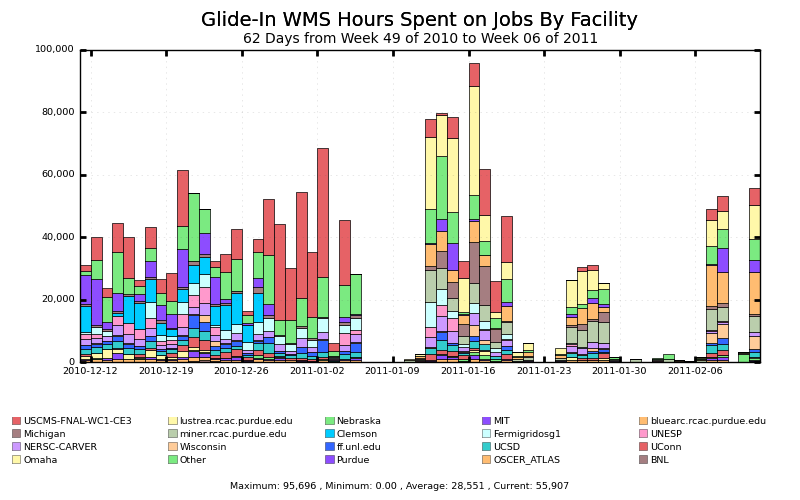
\includegraphics[scale=0.5]{images/glidein_hours_bar_smry}
\caption{Snapshot of Accounting of the HCC Campus Grid}
\label{fig:hccaccounting}
\end{center}
\end{figure}

Accounting on the execute resource side is very useful and is the current model in the OSG.  When a job is submitted in the OSG, it always passes through a gatekeeper on the local resource.  Accounting is done on the gatekeeper since it will see every OSG job running at the resource.

Unfortunately, due to the nature of flocking, accounting on the execute resources is more difficult on the HCC Campus Grid.  When flocking occurs, the submitter and the execute resource communicate directly, bypassing any gatekeeper.   The only way to keep accurate accounting data is to collect it from the worker nodes.  In the CGF installs, the accounting would need to run on the pilot submitted to PBS.  Condor does not support creating Gratia compatible records on the execute site.  This will be left for future work.


\subsection{Data Management}
Data management has been done differently by each campus.  GLOW maintains a global AFS that is available on every worker node.  Purdue has a few large file systems that worker nodes can access.  FermiGrid has a global Network File System (NFS) space for data.  Oxford grid uses the Storage Resource Broker (SRB) and a single vault.

The OSG promotes staging data to a nearby storage element which is difficult for individual users to implement.  Normally a user will stage data to the gatekeeper, then transfer it to the execute host.  This can lead to several bottlenecks when transferring large amounts of data to the gatekeeper.

HCC does not have a central file system, and instead uses Condor file transfer.  This method has several benefits:

\begin{itemize}
\item Removes the gateway as a bottleneck by transferring files directly from submitter to execute host.
\item Reduces dependence on the gateway as a failure point.  The gateway could terminate or become unavailable while a job is running and Condor would still be able to transfer back the output, and even start another job.
\item Reduces the work that the gateway needs to perform.  The authentication and authorization are done by the execute and submission hosts.
\item Not dependent on the reliability or bandwidth of the shared file system.  The submitter is relatively unaffected by other users that are not running on the same submission host.
\end{itemize}

There are some downsides to this approach.  The largest is the reliance on the submitter machine.  If the submitter becomes unavailable, all data transfers will fail.  I believe this is an acceptable risk; if the machine is unavailable for more than the 15 minute job lease, all jobs from the submitter will stop.

\subsection{Updated table of Campus Grid Attributes}
\begin{table}[h!t]
\centering
\small
\begin{tabular}{ | p{50pt} | | p{68pt} | p{54pt} | p{60pt} | p{50pt} | p{60pt} |}
\hline
Grid & Trust & Job & Resource & Accounting & Data \\ 
& Relationship & Submission & Independence & & Management \\
\hline \hline
Virginia &  LDAP/PKI  & None \mbox{Described} & Strict & Central & None     \\ \hline
Oxford & Kerberos/PKI & Central & Central \mbox{Submission} & Custom & SRB  \\ \hline
Purdue & Host &  Distributed & Strict & Custom & Condor Transfer  \\ \hline
GLOW &  Host & Distributed & Strict & None &  Condor Transfer \\ \hline
FermiGrid & PKI & Central & Strict & OSG \mbox{Gratia} & Central File System  \\ \hline
OSG & PKI  & Distributed & Strict & OSG \mbox{Gratia} & Distributed \\ \hline
HCC & Campus Defined & Distributed & Strict & OSG \mbox{Gratia} & Condor Transfer \\ \hline
\end{tabular}
\caption{Updated Campus Grid Attributes} \label{tab:updatedcampusgridoverview}
\end{table}

The Campus Grid attributes with HCC are shown in Table \ref{tab:updatedcampusgridoverview}.  


\section{Usage}

\begin{figure}[h!tb]
\begin{center}
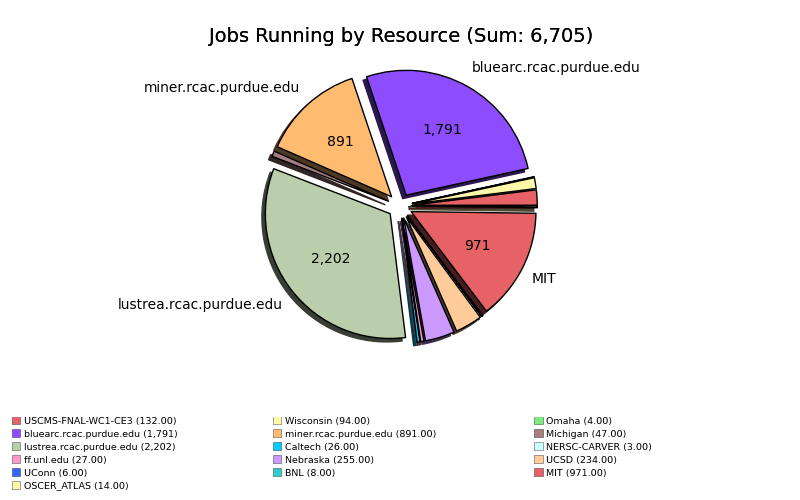
\includegraphics[scale=0.6]{images/allsites}
\caption{Snapshot of Usage of the Extended HCC Campus Grid}
\label{fig:snapshothccgrid}
\end{center}
\end{figure}

In Figure \ref{fig:snapshothccgrid} one can see a snapshot of production jobs submitted from the GlideinWMS interface host running on the HCC Campus Grid.  Note the total number of jobs running, (8612):  this is larger than the total number of cores in any single Nebraska cluster and larger than the sum total of all cores managed by HCC (8000).  

A description of the resources shown in the picture follows.
\begin{itemize}
\item \textbf{Local Resources}: ff.unl.edu, prairiefire.unl.edu
\item \textbf{Peered campus resources}: bluearc.rcac.purdue.edu, lustrea.rcac.purdue.edu, miner.rcac.purdue.edu
\item \textbf{OSG through GlideinWMS}: USCMS-FNAL-WC1-CE3 (Fermilab), Omaha (Globus submission to Firefly), Michigan, Caltech, NERSC-CARVER, \mbox{Nebraska} (Nebraska Tier 2), UCSD, UConn, BNL (Brookhaven), Wisconsin, MIT, \\ OSCER\_ATLAS (OU).
\end{itemize}

Another observation is the number of jobs running at the peered campus, Purdue.   Purdue has large resources and peering with them has significantly increased the available resources to Nebraska researchers.  As described in Figure \ref{fig:campusgrid}, the submitter first looks at local resources \texttt{ff.unl.edu} (CGF) and \texttt{prairiefire.unl.edu} (Condor).  Both had few resources available, so the submitter moved onto the OSG and peered campuses.  The peered campus had many resources available (especially \texttt{lustrea.rcac.purdue.edu}).  Sites in the OSG were able to start jobs (see Fermilab, Wisconsin, MIT).  

Currently, the campus grid factory is used in production only on Firefly at Nebraska.  It is currently being run in test environments at the National Center for Supercomputing Applications (NCSA) \cite{ncsa}.  At the NCSA, researchers from the Renaissance Computing Institute \cite{renci} have installed the CGF to flock from their submission host at their institution.  Campus grids such as Louisiana Tech and the Sunshine Grid in Florida are experimenting with the framework.




\chapter{Conclusions and Future Work}
\label{sec:Conclusion}

The framework described in this thesis creates a grid of clusters that transparently overflow to each other.  The grid can overflow to national cyberinfrastructure and peered campuses through production interfaces.  The CGF was developed to connect a PBS cluster into the Condor campus grid.  The HCC campus grid is a production grid, running many users' jobs.

The framework includes many components developed by external organizations such as BLAHP (gLite), Condor (University of Wisconsin--Madison), and GlideinWMS (Fermilab).  These components are glued together by Condor and the CGF to create a uniform grid.

By using production components from other grids, I was able to build a framework that integrates all clusters on the campus into the HCC Campus Grid, as well as overflow to the regional and national cyberinfrastructure.  Further it develops the idea of a tiered model: the framework prefers to run jobs locally before expanding to the campus, and finally overflowing to regional and national grids.

Further refinement of data management and accounting are left for future work.  Data management has proven difficult in the OSG, and it is no different in a campus grid.  Transparent access to storage has been a goal for the OSG and major collaborators for some time.  CMS and ATLAS are moving towards cache--based data distribution methods \cite{campana2011commissioning}.  The campus grids should follow this model as well,  whether this is as simple as using web caching, or more complicated such as utilizing Xrootd \cite{dorigo2005xrootd} for data distribution.  Similar to the BLAHP, Condor, and GlideinWMS, the components developed by the large experiments CMS and ATLAS should be adapted for use on the campus grid.  The work done by the large experiments to adapt the these components to their grids is much larger than the effort available for campus grids.  

Accounting also will be improved in the future.  It is important for resource owners to determine the hours given to external entities.  This can be accomplished with the execution side reporting usage.  This model is not used in the OSG and will need to be developed separately.

The campus grid ideas outlined in this thesis are being used in other states for their campus grids.  Institutions such as Florida State and Louisiana Tech are installing the software and evaluating it for their campus grids.  The Campus Grid area of the OSG will include the software and ideas developed here.




\backmatter

\bibliographystyle{plain}
\bibliography{DerekWeitzelThesis}



\end{document}

\endinput

